 \documentclass[10pt,journal,compsoc]{IEEEtran}
\usepackage{alltt}
\usepackage{multirow}
\usepackage{graphicx}
\usepackage{color}
\usepackage[labelfont=bf,textfont={bf}]{caption}
\usepackage{subcaption}
\usepackage{pifont}% http://ctan.org/pkg/pifont
\usepackage{boxedminipage}
\usepackage{notoccite}
\usepackage{array}
\newcolumntype{C}[1]{>{\centering\let\newline\\\arraybackslash\hspace{0pt}}m{#1}}
\usepackage{enumerate}
\usepackage{booktabs}
% \usepackage{minted}
\usepackage[framemethod=tikz]{mdframed}
\usepackage{lipsum}
\usetikzlibrary{shadows}
\usepackage{mathtools}
 \usepackage{paralist}
 \definecolor{light-gray}{gray}{0.80}
\usepackage{graphics}
\usepackage[shortlabels]{enumitem}
%\usepackage{balance}
\usepackage{dblfloatfix}

%\usepackage{hyperref}
%\usepackage{cleveref}
\usepackage{colortbl}
\newmdenv[
  tikzsetting= {fill=light-gray},
  linewidth=1pt,
  roundcorner=0pt, 
  shadow=false
]{myshadowbox}
\usepackage{colortbl} 
\usepackage{subcaption}
\usepackage{blindtext, graphicx}
\usepackage{textcomp}
\usepackage{mathtools}
\usepackage[hidelinks]{hyperref}
\usepackage{amsmath}
\usepackage{amsfonts}
\usepackage{caption}
\usepackage{color}
\usepackage[final]{listings}
\usepackage{graphicx} 
\usepackage{multirow}
\usepackage{balance}
\usepackage{picture}
\usepackage{relsize}
\usepackage{multicol}
\usepackage{soul}
\usepackage{enumitem}
\setitemize{noitemsep,topsep=0pt,parsep=0pt,partopsep=0pt,leftmargin=*}
\setenumerate{noitemsep,topsep=0pt,parsep=0pt,partopsep=0pt,leftmargin=*}
\DeclarePairedDelimiter\abs{\lvert}{\rvert}%
\usepackage{array}
\usepackage{makecell}
\usepackage{bigstrut}
\newcommand{\tion}[1]{\S\ref{sect:#1}}
\newcommand{\fig}[1]{Figure~\ref{fig:#1}}
\newcommand{\tab}[1]{Table~\ref{tab:#1}}

\newcommand{\tbl}[1]{Table~\ref{tbl:#1}}
\definecolor{comment_color}{rgb}{0.5, 0, 1}
\definecolor{steel}{rgb}{0.1, 0.3, 0.5} 
\newcommand{\cmark}{\ding{51}}%
\newcommand{\xmark}{\ding{55}}%
\newcommand{\todoc}[2]{{\textcolor{#1}{\textbf{[[#2]]}}}}
\newcommand{\todobrown}[1]{\todoc{green}{\textbf{[[#1]]}}}
\newcommand{\todoblue}[1]{\todoc{blue}{\textbf{[[#1]]}}}
\newcommand{\todoorange}[1]{\todoc{cyan}{\textbf{[[#1]]}}}
\newcommand{\todored}[1]{\todoc{red}{\textbf{[[#1]]}}}
\newcommand{\rahul}[1]{{\textcolor{steel}{#1}}}
\newcommand{\bi}{\begin{itemize}}
\newcommand{\ei}{\end{itemize}}
\usepackage[
 pass,% keep layout unchanged
 % showframe,% show the layout
]{geometry}
\usepackage[skins]{tcolorbox}
\usepackage{verbatim}
\usepackage{algorithm}
\usepackage{algorithmicx}
\usepackage{algpseudocode}
\usepackage[export]{adjustbox}
\usepackage{mathtools}
\setlength{\belowcaptionskip}{-10pt}
\renewcommand{\footnotesize}{\scriptsize}
\renewcommand{\algorithmicrequire}{\textbf{Input:}}
\renewcommand{\algorithmicensure}{\textbf{Output:}}
\definecolor{lightgray}{gray}{0.8}
\definecolor{LightCyan}{rgb}{0.88,1,1}
\definecolor{darkgray}{gray}{0.7}
\definecolor{Gray}{rgb}{0.88,1,1}
\definecolor{Gray}{gray}{0.85}
\definecolor{Blue}{RGB}{0,29,193}
\definecolor{MyDarkBlue}{rgb}{0,0.08,0.45} 
\definecolor{pink}{RGB}{231,95,110}
\definecolor{lightergray}{rgb}{0.85, 0.85, 0.85}
\definecolor{darkgray}{rgb}{0.47, 0.47, 0.47}
\definecolor{lightestgray}{rgb}{0.95, 0.95, 0.95}
\definecolor{ao(english)}{rgb}{0.0, 0.5, 0.0}
% \frenchspacing
\lstset{
  language=Python,
  basicstyle=\sffamily\fontsize{2.5mm}{0.8em}\selectfont,
  breaklines=true,
  prebreak=\raisebox{0ex}[0ex][0ex]{\ensuremath{\hookleftarrow}},
  frame=l,
  showtabs=true,
  columns=fullflexible,
  showspaces=false,
  showstringspaces=false,
  keywordstyle=\color{pink}\bfseries\sffamily\fontsize{2.8mm}{0.6em},
  emph={train, predict, add_samples, FindBellwether, BEETLE, get_cost, sample, get_perf, remove_non_bellwethers, LinearTransform, GPTransform,General,get_featrures,BIRCH,bellwether,get_bellwethers,O(N)}, 
  emphstyle=\bfseries\color{blue!50!black} ,
  stringstyle=\itshape\color{black!50},
  commentstyle=\color{red!50!black}\it,
  numbers=left,
  captionpos=t,
  escapeinside={\%*}{*)}
}

\newcommand{\response}[1]{\textcolor{blue}{#1}}
\usepackage[tikz]{bclogo}
\newenvironment{RQ}[1]%
{\noindent\begin{minipage}[c]{\linewidth}%
\begin{bclogo}[couleur=gray!20,%
                arrondi=0.1,logo=\bctrombone,% 
                ombre=true%
                ]{{\small  ~#1}}}%
{\end{bclogo}\vspace{2mm}\end{minipage}}

\usepackage{fancyvrb}
\fvset{%
fontsize=\small,
numbers=left
}
\newcommand{\be}{\begin{enumerate}}
\newcommand{\ee}{\end{enumerate}}
\newcommand{\eq}[1]{Equation~\ref{eq:#1}}

%%% graph
\newcommand{\crule}[3][darkgray]{\textcolor{#1}{\rule{#2}{#3}}}
\newcommand{\quartex}[3]{
\begin{picture}(13,6)%1
  {
   \color{black}
    \put(#3,3)
    {\circle*{4}}
    \put(#1,3)
    {\line(1,0){#2}}
  }
\end{picture}
}
\definecolor{lightgray}{gray}{0.7}
\tikzstyle{highlighter} = [lightgray, line width = \baselineskip]
\usepackage{wrapfig}
\newcounter{highlight}[page]
\newcommand{\tikzhighlightanchor}[1]{\ensuremath{\vcenter{\hbox{\tikz[remember picture, overlay]{\coordinate (#1 highlight \arabic{highlight});}}}}}
\newcommand{\bh}[0]{\stepcounter{highlight}\tikzhighlightanchor{begin}}
\newcommand{\eh}[0]{\tikzhighlightanchor{end}}
\AtBeginShipout{\AtBeginShipoutUpperLeft{\ifthenelse{\value{highlight} > 0}{\tikz[remember picture, overlay]{\foreach \stroke in {1,...,\arabic{highlight}} \draw[highlighter] (begin highlight \stroke) -- (end highlight \stroke);}}{}}}


\newcommand{\squishlist}{
 \begin{list}{$\bullet$}
 { \setlength{\itemsep}{0pt}
   \setlength{\parsep}{3pt}
   \setlength{\topsep}{3pt}
   \setlength{\partopsep}{0pt}
   \setlength{\leftmargin}{1.5em}
   \setlength{\labelwidth}{1em}
   \setlength{\labelsep}{0.5em} } }

\newcommand{\squishlisttwo}{
 \begin{list}{$\bullet$}
 { \setlength{\itemsep}{0pt}
  \setlength{\parsep}{0pt}
  \setlength{\topsep}{0pt}
  \setlength{\partopsep}{0pt}
  \setlength{\leftmargin}{1em}
  \setlength{\labelwidth}{1.5em}
  \setlength{\labelsep}{0.5em} } }

\newcommand{\squishend}{
 \end{list} }

\newcommand{\specialcell}[2][c]{%
 \begin{tabular}[#1]{@{}c@{}}#2\end{tabular}}

\newcommand{\flash}{{\sc Flash}\xspace}
\usepackage{soul}
\usepackage{color}

\definecolor{awesome}{rgb}{1.0, 0.13, 0.32}


\usepackage{amsmath}
\definecolor{Gray}{gray}{0.95}
\definecolor{LightGray}{gray}{0.975}

\DeclareRobustCommand{\hlgreen}[1]{{\sethlcolor{green}\hl{#1}}}
\DeclareRobustCommand{\hlyellow}[1]{{\sethlcolor{yellow}\hl{#1}}}
\DeclareRobustCommand{\hlred}[1]{{\sethlcolor{awesome}\textbf{\hl{#1}}}}


%% reviewing
\newcommand{\blue}[1]{{\color{blue}{#1}}}
\newcommand{\review}[1]{\vspace{3mm}{\noindent\textit{#1}}\vspace{3mm}}
\newcommand{\reponse}[1]{\noindent{#1\\}}
\newcommand{\todo}[1]{\textbf{\color{red}{#1}}}
\newcommand{\subsect}[1]{\SS\ref{subsect:#1}}

%% Response text prefix
\newcommand{\respto}[1]{
\fcolorbox{black}{black!15}{%
\label{resp:#1}%
\bf\scriptsize R{#1}}}

%% Response text prefix
\newcommand{\bareresp}[1]{
\fcolorbox{black}{black!15}{%
\bf\scriptsize R{#1}}}

%% Cite responses
\newcommand{\citeresp}[1]{%
{(see }\fcolorbox{black}{black!15}{%
\bf\scriptsize R{#1}}~{{on page \pageref{resp:#1})}}}%
\usepackage{cite}
% \usepackage[switch, pagewise]{lineno}
% \linenumbers

\newenvironment{steelblue}
{\color{steel}}
{\color{black}}

\newenvironment{result}
{\vspace{0.15cm}
\noindent\begin{minipage}{\linewidth}
\begin{center}
\arrayrulecolor{lightergray}
\begin{tabular}{|p{0.95\linewidth}|}
\hline%
\rowcolor{lightergray}%
\textbf{Result:}~%
}
{\\\hline
\end{tabular}
\end{center}
\end{minipage}
\vspace{0.15cm}
}

\newenvironment{goal}
{\vspace{0.15cm}
\noindent\begin{minipage}{\linewidth}
\begin{center}
\arrayrulecolor{black}
\begin{tabular}{|p{0.95\linewidth}|}
\hline\rowcolor{lightestgray}}
{\\\hline
\end{tabular}
\end{center}
\end{minipage}
\vspace{0.15cm}
}

\newcommand{\quart}[4]{\begin{picture}(100,6)%1
{\color{black}\put(#2,3){\color{black}\circle*{4}}\put(#1,3){\line(1,0){#3}}}\end{picture}}
\newcommand{\quartr}[4]{\begin{picture}(100,6)%1
{\color{black}\put(#2,3){\color{red}\circle*{4}}\put(#1,3){\line(1,0){#3}}}\end{picture}}
\newcommand{\quartx}[4]{\begin{picture}(100,1)%1
{\color{black}\put(\numexpr #2 * 6  \relax,3){\color{red}\circle*{4}}\put(\numexpr #1*6 \relax ,3){\line(1,0){\numexpr #3*6 \relax}}}\end{picture}}

\begin{document}
\title{  How to Find GENERAL    Defect Prediction Models  \\
Amidst Hundreds of    Software Projects}


\author{Suvodeep Majumder, Rahul Krishna and Tim Menzies,~\IEEEmembership{IEEE Fellow}
%\affiliation{Computer Science, NCSU, USA, North Carolina}  
%\email{[smajumd3,rkrish11]@ncsu.edu, tim@ieee.org}

\IEEEcompsocitemizethanks{\IEEEcompsocthanksitem S, Majumder, R. Krishna and  T. Menzies are with the Department
of Computer Science, North Carolina State University, Raleigh, USA.\protect\\
E-mail:[smajumd3,rkrish11]@ncsu.edu, tim@ieee.org}}
 

% The paper headers
\markboth{IEEE Transactions on Software Engineering, submitted Oct `19}{Majumder \MakeLowercase{\textit{et al.}}: GENERAL: Scaling Transfer Learning to 100s of Projects}

\IEEEtitleabstractindextext{%
\begin{abstract}
\respto{2-22}{\color{blue} When one   exemplar project, which we call the ``bellwether'', offers the best prediction
then
it can be used to offer prediction for
many other projects. Such bellwethers can be used to make quality predictions about new projects, even before there is much experience with those new projects.}
% Such general conclusions   simplifies     software quality policies since the list of quality problems, and their mitigations, is static). Also such general conclusions simplify the design and delivery
% of training programs since, as long as the bellwether offers best advice,
% then  ``best practices'' will remain  now constant.
% Lastly, bellwethers simplify tool development
% since, using the advice from the bellwether,  it is clear where it is most cost-effective to buy/build tools to mitigate
% for software quality issues.

But  existing  methods  for  bellwether  transfer  are  very slow.  When  applied  to  the  697  projects  studied  here,  they took  60  days  of  CPU  to  find  and  certify  the  bellwethers
Hence,  we  propose GENERAL:  a novel bellwether detection algorithm based on
  hierarchical clustering. At each level within a tree of clusters, one bellwether is computed from sibling projects, then promoted up the tree. 
This hierarchical method is a scalable approach to learning effective models from very
large data sets. 
For example, for nearly 700 projects,
the defect prediction models generated from GENERAL's bellwether  
were  just as good as those found via  standard methods.   


% Having shown that it is
% possible to transfer lessons learned across
%  100s of projects, our future work
%  will be to  achieve ``mega-transfer'';
%  i.e. to transfer lessons learned between
%  1000s to 10,000s of projects. 
 
 

\end{abstract}

\begin{IEEEkeywords}
Transfer Learning, Bellwether, Defect Prediction, Software Analytics. 
\end{IEEEkeywords}}



% make the title area
\maketitle

\IEEEdisplaynontitleabstractindextext
\IEEEdisplaynontitleabstractindextext


\ifCLASSOPTIONcaptionsoff
 \newpage
\fi

\section{Introduction}


%   After a decade of intensive research into automated software analytics, what general principles have we learned? While that work has generated specific results about specific projects~\cite{Bird:2015,menzies2013software}, it has failed (so far) to deliver general principles that are demonstrably useful across many projects~\cite{menzies2013guest} (for an example of how {\em more} data can lead to {\em less} general conclusions, see below in {\S}2a).

% Is that the best we can do?

% How should we reason about software quality?  Should we use  general models that hold over many projects? Or must we use an ever-changing set of ideas that are   continually adapted to the task at hand? 
% Or does the truth lie somewhere in-between?  
% To say that another way:
% \bi
% \item
% Are there general principles we can use to guide project management, software standards, education,   tool development, and legislation about software? 
% \item
% Or is  software engineering some ``patchwork quilt'' of ideas and methods where it only makes sense to reason about specific, specialized, and small sets of  projects?
% \ei
% If the latter were true then
%  then there would be no stable conclusions about what is best practice for SE   (since those best practices would keep changing as we move from project to project). As discussed in section~\ref{sec:Motivation}, such conclusion instability has   detrimental implications for {\em generality, trust, insight, training}, and {\em tool development}.
 
\respto{1-3}{\color{blue}Researchers and industry practitioners makes use of software analytics for many tasks to access software quality, such as:
\bi
\item Predicting if a submitted code is likely to buggy or not.
\item Improving code quality by detecting code smells.
\item Issue lifetime estimation to enable effective development and maintenance of their software systems.
\ei

Large organizations and many open source communities uses data-driven decision making, where they learn using large scale data analysis on historical data available to them. With large quantity of data available to them, how should they reason about software quality? Should they use  general models that hold over many projects? Or must they use an ever-changing set of ideas that are   continually adapted to the task at hand? If the latter were true then there would be no stable conclusions about what is best practice for SE   (since those best practices would keep changing as we move from project to project). As discussed in section~\ref{sec:Motivation}, such conclusion instability has   detrimental implications for {\em generality, trust, insight, training}, and {\em tool development}.}
%One  explanation for the limited conclusions (so far) from automated analytics is  {\em how much} data we are using for analysis. A typical software analytics research paper uses less than a few dozen projects  (exceptions: see~\cite{krishna18a, zhao17, agrawal18}). Such small samples can never represent something as diverse as software engineering. 

Finding general lessons across multiple projects is a complex task.
A new approach, that shows much promise, is the ``bellwether'' method for transferring conclusions between projects~\cite{krishna2018bellwethers,krishna16a,mensah18z,mensah2017stratification,mensah2017investigating}. \respto{1-1}{\color{blue} ``bellwether'' is a project from a community of N projects, whose data yields the best analytic (i.e. defect prediction, effort estimation etc) on all others.} (the bellwether is the  leading sheep of a flock, with a bell on its neck).  This method:
\bi
\item Finds a  ``bellwether'' project that is exemplar for the rest;
\item Draw conclusions from  that project.
\ei
This approach has been successfully applied to defect prediction, software effort estimation, bad smell detection, issue lifetime estimation, and configuration optimization. As a method of transferring lessons learned from one project to another, bellwethers have worked better than the Burak filter~\cite{turhan09}, Ma et al.~\cite{Ma2012}'s transfer naive Bayes (TNB); and Nam et al.  TCA  and TCA+, algorithms~\cite{Nam13,Nam2015}.

%In terms of {\em transfer} and {\em lessons learned},  such bellwethers have
 % tremendous practical significance. 
  When new projects arrive, then even before there is much experience with those new projects,  lessons learned from other projects can be applied to the new project (just by studying the bellwether),
 Further, \respto{2-2}{\color{blue} since the bellwether is an exemplar projects for the community of N projects seen so far},
 %since the bellwether is similar to the other models
 then when new projects appear, \respto{2-3}{\color{blue} bugs can be localized for that project} even before there is an extensive experience base within that particular project (again, just by studying the bellwether).
 %That is, bellwethers can be queried  to find general lessons about (a)~major quality issues;
 %or (b)~best practices to avoid quality problems;
 %or (c)~cost-benefit justifications for buying or building tools can be made stable across a large number 
 %of projects. 
 

But existing  methods for bellwether transfer are very slow. When applied to the 697 projects studied here, they took 60 days of CPU to find and certify the bellwethers. There are many reasons for that including how the models were certified (20 repeats  with different train/test sets)
and the complexity of the analysis procedure (which includes fixing class imbalance and feature selection). But the major cause of this slow down was that those   methods  required an $O(N^2)$ comparison between   $N=697$ projects.



This paper reports a novel approach  that improves on existing bellwether methods.
%dramatically improves on existing bellwether methods.
 Our GENERAL  method  uses hierarchical clustering model to recursively divide a large number of projects into smaller clusters. Starting at the leaves of that tree of clusters, GENERAL finds the    bellwethers within sibling projects. That bellwether is then promoted up the tree. The output of GENERAL is the project promoted to the top of the tree of clusters. 
 
 This paper evaluates the model built from the project   found by GENERAL. 
 We will find that  the predictions
 from this model  are as good, or better,
 than those found  via ``within'' learning (where models are trained and tested on local data)
 or ``all-pairs'' learning (where models are found after building models from all pairs of projects).
   That is
\begin{quote}
{\em 
Learning from many other projects can be better than learning just from your own local project data.
}\end{quote}
GENERAL's clustering methods divide $N$ projects into $m$ groups. In that space,   GENERAL only needs
to compare $O(m*(N/m)^2)$  projects to find the bellwether. Theoretically and empirically, 
this means GENERAL will scale up much better than traditional   methods. For example: This paper applies GENERAL and traditional $O(N^2)$ bellwether to 697 projects. GENERAL and the traditional approach terminated in 1.5 and 72 hours (respectively).
% \bi
% \item
% This paper applies GENERAL and traditional $O(N^2)$ bellwether to 697 projects.
% GENERAL and the traditional approach terminated in 1.5 and 72 hours (respectively).

% \item 
%  Figure~\ref{fig:cost} shows a hypothetical cost comparison in AWS between standard bellwethers and   GENERAL when running for 100 to 1,000,000 projects. Note that GENERAL
%  is inherently more scalable.
%  \ei
% \begin{figure}[!t]
%     \centering
%     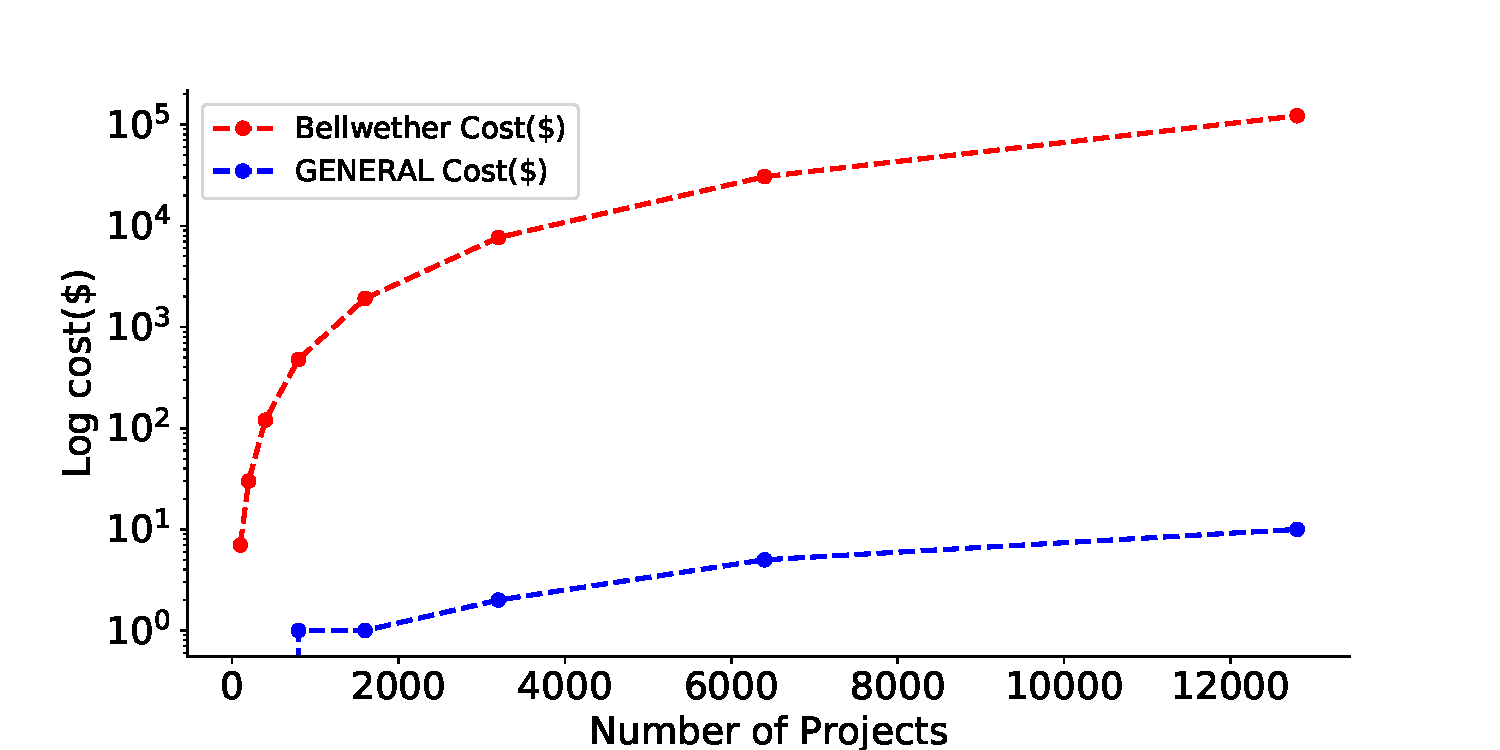
\includegraphics[width=\linewidth]{figs/cost.pdf}
%     \caption{Hypothetical cost comparison between GENERAL and default Bellwether.}
%     \label{fig:cost}
% \end{figure} 
Using GENERAL, we can  explore these research questions:
            \respto{1-6}
            
            {\color{blue}
            \textbf{RQ1}:  How slow is conventional bellwether method?
            
            \begin{RQ}{
               Conventional bellwether method as proposed by krishna et al~\cite{krishna2018bellwethers,krishna16a} uses a $ O(N^2) $ comparisons to find the ``bellwether'' among a community of N (697 projects in this experiment) projects. In this experiment the conventional bellwether method used almost 72 hours to find the ``bellwether''.}
            \end{RQ}
            
            \textbf{RQ2}:  How fast is new bellwether method aka GENERAL?
            
            \begin{RQ}{
               The new bellwether method (GENERAL), which is a combination of hierarchical clustering and bellwether method took around 1.5 hours find a ``bellwether''.}
            \end{RQ}
            
            }

 
            \textbf{RQ3}:   Can hierarchical clustering tame the complexity of bellwether-based reasoning?
            
            \begin{RQ}{
               Theoretically and empirically, the 
hierarchical
reasoning on GENERAL performs much
faster than standard bellwether methods.}
            \end{RQ}

         

 
           \noindent \textbf{RQ4}:  Is this faster bellwether effective?
            
            \begin{RQ}{
                Measured in terms of predictive performance,
the effectiveness of hierarchical bellwethers
is very similar to local learning
(and these two methods are more effective
than the other options explored here).}
            \end{RQ}
        
       \noindent 
            \textbf{RQ5}: Does learning from too many projects have detrimental effect?
            
            \begin{RQ}{
            Assessed in terms of {\em recall},
it is better to learn bellwethers from more data rather than less.
But assessed in terms of {\em false alarms}, 
while learning bellwethers
from many projects is useful, it is possible to learn from too much data.}
            \end{RQ}
            
         \noindent 
            \textbf{RQ6}: What exactly did we learn from all those projects?
            
            \begin{RQ}{
                The importance of many key features is not apparent at the local
level. To fully appreciate the critical impact on defects
of class interface design,  it is necessary to conduct
a global analysis across hundreds of projects. }
            \end{RQ}

    
\noindent Overall, the  contributions of this paper are
\bi

\item \textbf{Hierarchical bellwethers for  transfer learner:} We
offer a  novel hierarchical clustering    bellwether algorithm  called GENERAL  (described in section~\ref{GENERAL}) that
finds bellwether in hierarchical clusters, then promotes those bellwether to upper levels
The final  project that is promoted to the root of the hierarchy is returned as  ``the'' bellwether.

\item \textbf{Showing inherent generality in SE:}
In this study we discover a source data set for transfer learner from a large number of   projects, hence proving generality in the SE datasets (where some datasets can act as exemplars for the rest of them for defect prediction).



\item \textbf{ Lessons   about software quality that are general
to hundreds of software projects:}
  As said above,    in  this sample of  697  projects,  we find that code  interface issues are the dominant factor on software defects. 
  
  
\item \respto{1-5h}{\color{blue}\textbf{ Replication Package:} We have made available a  replication package\footnote{\href{http://tiny.cc/bellwether}{http://tiny.cc/bellwether}} . The  replication package consists of all the datasets used in this paper, in addition to mechanisms for computation of other statistical measures.}

\ei
The rest of this paper is structured as follows. Some background and related work are discussed in section~\ref{sec:literature}. Our algorithm GENERAL is described in section~\ref{GENERAL}. Data collection and experimental setup are in section~\ref{sec:Data Collection}. Followed by evaluation criteria in section~\ref{eval} and performance measures in section~\ref{sec:Measures}. The results and answers to the research questions are presented in section~\ref{sec:results}, which is followed by threats to validity in section~\ref{sec:validity}. Finally the conclusion is provided in section~\ref{sec:concl}.



\section{Motivation}
\label{sec:motivation}

\subsection{Why Seek Generality?}
\label{sec:Motivation}
There are many reasons to seek stable general conclusions in software engineering. If our conclusions about best practices for SE projects keep changing, that will be detrimental to generality, trust, insight, training, and tool development.

\textbf{Generality:} Data science for software engineering cannot be called a ``science'' unless it makes general conclusions that hold across  multiple  projects. If we cannot offer general rules across a large number of software projects, then it is   difficult to demonstrate such generality.

\textbf{Trust:} Hassan~\cite{Hassan17} cautions that managers lose faith in software analytics if its models keep changing since  the assumptions used to make prior policy decisions may no longer hold.

\textbf{Insight:} Kim et al.~\cite{Kim2016}, say  that the aim of software analytics is to obtain actionable insights that help practitioners accomplish software development goals. For Tan et al.~\cite{tan2016defining}, such   insights  are a core deliverable. Sawyer et al. agree, saying that  insights are the key driver for businesses to invest in data analytics initiatives~\cite{sawyer2013bi}. Bird, Zimmermann, et al.~\cite{Bird:2015} say that such  insights occur when users reflect, and react, to the output of a model generated via software analytics. But if  new models keep being generated in new projects, then that exhausts the ability of  users to draw insight from  new data.

\textbf{Training:} Another concern is what do we train novice software engineers or newcomers to a project? If our models are not stable, then it hard to teach what factors  most influence software quality.

\textbf{Tool development:} Further to the last point--- if we are unsure what factors most influence quality, it is difficult to design and implement and deploy tools that can successfully improve that quality.


% \begin{figure}[!t]
%     \centering
%     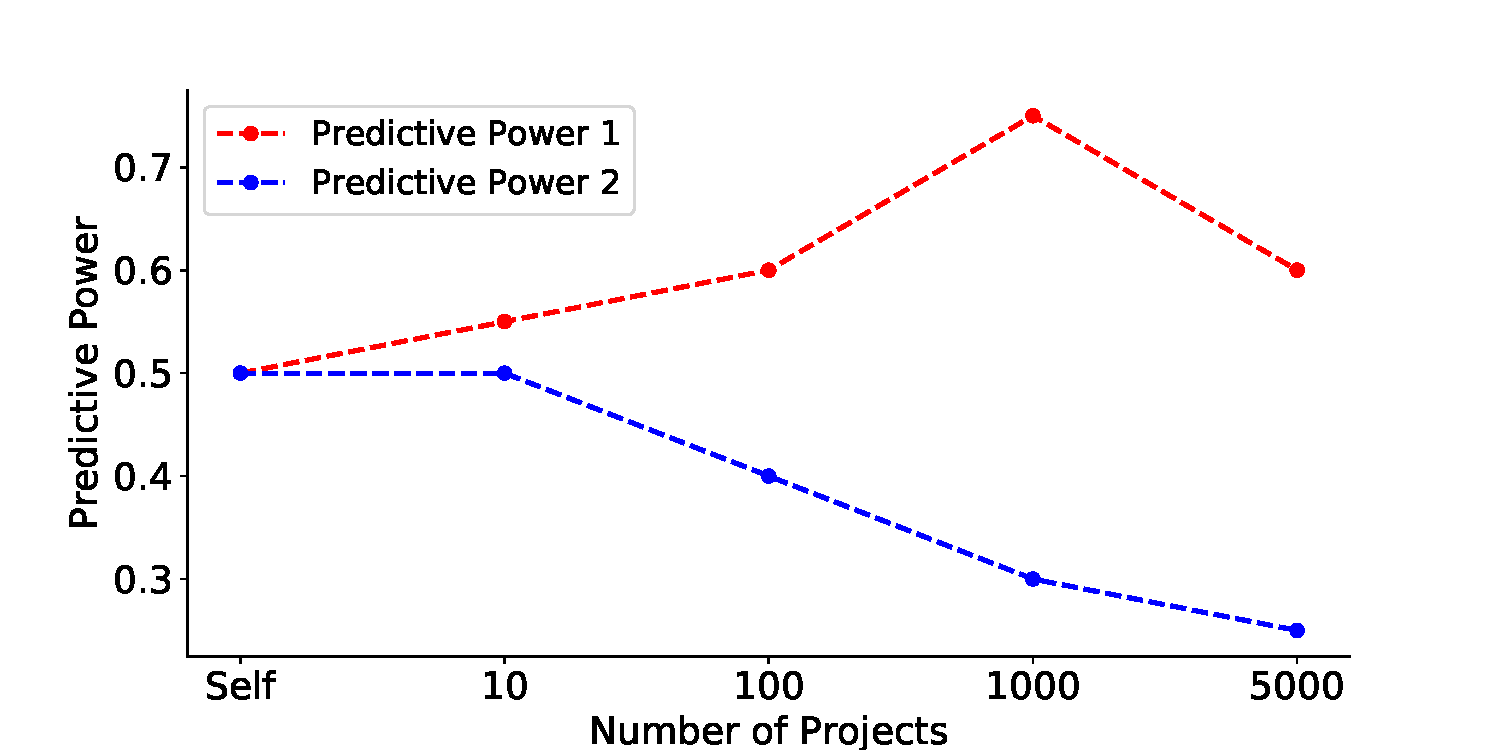
\includegraphics[width=\linewidth]{figs/predictive_power.pdf}
%     \caption{Two hypothetical results about how training set size might effect the efficacy of quality prediction for software projects.}
%     \label{fig:predictive_power}
% \end{figure}



\subsection{Why Shun Generality?}
Just to balance the above argument,
we add that   sometimes it is possible to learn from {\em too much data}.
Petersen and Wohlin~\cite{Petersen2009} argue that for empirical SE, context matters. That is, they would predict that one model  will \underline{not}  cover all  projects and that tools that report  generality  over many software projects need to also know the {\em communities} within which those conclusions   apply. Hence, this work divides into (a)~automated methods for finding sets of projects in the same {\em community}; and (b)~within each {\em community}, find the model that works best. 

\respto{2-12}{\color{blue} The {\em size} of the communities found in this way would have a profound impact on how we should reason about software engineering. Consider in this experiment of 697 projects, we build a set of defect predictor by learning bellwether from smalls cluster of $\approx10$ projects,  medium clusters of $\approx100$ projects, a large cluster containing $\approx600$ projects and a self test. In this scenario if we see the defect prediction models build  using bellwethers from medium set of clusters works better than set smalls clusters as well as the large cluster, then in this case, while we could not offer a single model that covers {\em all} of SE, we could offer a handful of models, each of which would be relevant to project clusters. While if we see only self test works in this case and learning from more projects makes quality predictions worse which means the our projects break up into ``communities'' of size one. In this case,  (a)~principles about what is ``best practice'' for different software projects would be constantly changing (whenever we jump from small community to small community); and (b)~the generality issues would be becoming open and urgent concerns for the SE analytics community.}

In summary, the above two sections lead to our  research question {\bf  RQ5}:
does learning from too many projects have detrimental effects. Later in this
paper, we will return to this issue.


% The {\em size} of the communities found in this way would have a profound impact on how we should reason about software engineering. Consider the hypothetical results of Figure~\ref{fig:predictive_power}. The \textcolor{blue}{{\bf BLUE}} curve shows some quality predictor that (hypothetically) gets better, the more projects it learns from (i.e. higher levels in the hierarchical cluster). After about learning from 1000 projects, the \textcolor{blue}{{\bf BLUE}} curve's growth stops and we would say that community size here was around cluster size in level 1. In this case, while we could not offer a single model that covers {\em all} of SE, we could offer a handful of models, each of which would be relevant to project clusters at that level. 
% %Accordingly, we would say that there are many cases where  wisdom from prior projects can be readily applied to guide future projects and (b)~the generality issues raised are not be so pressing.

% Now consider the hypothetical \textcolor{red}{{\bf RED}} curve of Figure~\ref{fig:predictive_power}. Here, we see that (hypothetically)  learning from more projects makes quality predictions worse which means the our 10,000 projects break up into ``communities'' of size one. In this case,  (a)~principles about what is ``best practice'' for different software projects would be constantly changing (whenever we jump from small community to small community); and (b)~the generality issues would be becoming open and urgent concerns for the SE analytics community.

% In summary, the above two sections lead to our  research question {\bf  RQ4}:
% does learning from too many projects have detrimental effects. Later in this
% paper, we will return to this issue.


\section{Background and Related Work}
\label{sec:literature}
\subsection{Why Transfer Knowledge?}
\label{sec:related}

In this section, we ask ``Why even bother to transfer lessons learned between projects?''. In several recent studies ~\cite{bettenburg2012think, menzies2012local, posnett2011ecological} with readily-available data from SE repositories, numerous authors report the locality effect in SE; i.e. general models outperformed by specialized models localized to particular parts of the data.
For example.
Menzies et al. explored local vs global learning in defect prediction and effort estimation~\cite{menzies2012local}  and found that
 learning rules from specific local data was more
 effective than learning rules from the global space.
 
 
On the other hand,
Herbold et al.~\cite{herbold2017global}  offered an opposite conclusion.
In their   study regarding global vs local model for cross-project defect prediction,
they saw that  local models offered little to no improvement over models learned
from all the global data.
One explanation for this discrepancy  is the size of number of projects that they explored.
Menzies, Herbold et al. explored less than two dozen projects which raises issues of external validity in their conclusions. Accordingly, here,  we explore nearly 700 projects. As shown below, the results of this paper agree  more with Herbold et al. than  Menzies et al. since we show that one global model (learned from a single bellwether projects) does just as well as anything else.

Apart from the above discrepancy in research results, there are many other reasons to
explore learning from many projects. Those reasons   falls into four groups:

\textbf{(a) The lesson on big data is that that the {\em more} training data, the {\em better} the learned model:} Vapnik~\cite{vapnik14} discusses examples where models accuracy improves to nearly 100\%, just by training on $10^2$ times as much data. This effect has yet to be seen in SE data~\cite{menzies2013guest} but that might just mean we have yet to use enough training data (hence, this study). 

\textbf{(b) We need to learn from more data since there is very little agreement on what has been learned so far:} 
% Another reason to try generalizing across more SE data is that, among developers, there is little agreement on what many issues relating to software:
\respto{2-23}{\color{blue} Among developers,  there is little agreement on what is of importance relating to software quality and other aspects of the software development:}
\bi
    \item
    According to Passos et al.~\cite{passos11},  developers often  assume that the lessons they learn from a few past projects are general to all their future projects. They comment, ``past experiences were taken into account without much consideration for their context'' ~\cite{passos11}. 
	\item
	J{\o}rgensen \& Gruschke~\cite{Jo09} offer a similar warning. They report that the suppose software engineering ``gurus'' rarely use lessons from past projects to improve their future reasoning and that such poor past advice can be detrimental to new projects.~\cite{Jo09}.
    \item 
    Other studies have shown some widely-held views are   now questionable given new evidence. Devanbu et al. examined responses from 564 Microsoft software developers from around
	the world. They comment programmer beliefs can vary with each project, but do not necessarily
	correspond with actual evidence in that project~\cite{De16}. 
\ei
	
The good news is that using software analytics, we can correct the above misconceptions. If data mining shows that doing  XYZ is bug prone, then we could  guide developers to avoid XYZ. But will developers listen to us? If they ask ``are we sure  XYZ causes problems?'', can we say that we have mined enough projects to ensure that XYZ is problematic? 

\respto{2-24}{\color{blue} It turns out that developers are not the only one's confused about how various factors influence software projects. Much recent research calls into question  the ``established wisdoms'' of SE field. 

Here is a list of recent conclusions that contradict prior conclusions:}

\bi
    \item In stark contrast to  much prior research, pre- and post- release failures are not connected~\cite{fenton2000quantitative};
    
    \item Static code analyzers perform no better than simple statistical predictors~\cite{Fa13}; 
    
    \item The language construct GOTO, as used in contemporary practice, is rarely considered harmful~\cite{nagappan2015empirical};
    
    \item Strongly typed languages are not associated with successful projects~\cite{ray2014large};  
    
    \item Test-driven development is not any better than "test last"~\cite{fucci2017dissection};
    
    \item Delayed issues are not exponentially more expensive to fix~\cite{menzies2017delayed};
\ei
Note that if the reader disputes any of the above, then we ask how would you challenge the items on this list? Where would you get the data, from enough projects, to   successfully refute the above? And where would you get that data? And how would you draw conclusions from that large set? Note that the answers to these questions requires learning from multiple projects. Hence, this paper.

\textbf{(c) Imported data can be more useful than local data:} Another benefit of  importing data from other projects is that, sometimes, that imported data can be better than the local information. For example, Rees-Jones reports in one study that while building predictors
for Github close time  for open source projects~\cite{rees2017better} using data from other projects performs much better then building models using {\em local learning} (because there is better  information {\em there} than {\em here}).


\textbf{(d) When there is insufficient local data, learning from other projects is very useful:} When developing new software in  novel areas, it is useful to draw on the relevant  experience  from related areas with a larger experience base.This is particularly true when developers are doing something that is novel to them, but has been widely applied elsewhere
For example, Clark and Madachy~\cite{clark15} discuss 65 types of software they see        under-development by the US Defense Department in 2015.   Some of these types are very common (e.g. 22 ground-based communication systems) but other types are very rare (e.g. only  one avionics communication system). (e.g. workers on   flight avionics   might check for lessons learned from ground-based communications). Developers  working in an uncommon area (e.g. avionics communications) might want to transfer in lessons from more common areas (e.g. ground-based communication).

\subsection{ How to  Transfer Knowledge}
This     art of moving data and/or lessons learned from one project or another is {\em Transfer Learning}. When there is insufficient current data to apply data miners to learn defect predictors, transfer learning can be used to transfer lessons learned from other source projects S to the target project T .

Initial experiments with transfer learning offered very pessimistic results. Zimmermann et al.~\cite{zimmermann2009cross} tried to port models between two web browsers (Internet Explorer and Firefox) and found that cross-project prediction was still not consistent: a model built on Firefox was useful for Explorer, but not vice versa, even though both of them are similar applications. Turhan's initial experimental results were also very negative: given data from 10 projects, training on S = 9 source projects and testing on T = 1 target projects resulted in alarmingly high false positive rates (60\% or more). 

Subsequent research realized that data had to be carefully sub-sampled and possibly transformed before quality predictors from one source are applied to a target project. Transfer learning can have two variants - 

\bi
\item    
 \textbf{Heterogeneous Transfer Learning:} This type of transfer learning operates on source and target data that contain the different attributes~\respto{2-17}{\color{blue}\cite{jing2015heterogeneous,he2014towards,nam2017heterogeneous,cheng2016heterogeneous,yu2017feature}}.

\item
\textbf{Homogeneous Transfer Learning:} This kind of transfer learning operates on source and target data that contain the same attributes. This paper explores scalable methods for homogeneous transfer~\respto{2-17}{\color{blue}\cite{ma2012transfer,zimmermann2009cross,turhan2009relative,krishna2018bellwethers}}.
\ei
Another way to divide transfer learning is the approach that is followed. There are  2 approaches that are frequently used in many research: {\bf similarity-based approaches} and {\bf dimensional transforms}.

 \textbf{Similarity-Based Approaches:} In this approach we can transfer some/all subset of the rows or columns of data from source to target. For example, the Burak filter~\cite{turhan09} builds its training sets by finding the k = 10 nearest code modules in S for every $ t \in T $. However, the Burak filter suffered from the all too common instability problem (here, whenever the source or target is updated, data miners will learn a new model since different code modules will satisfy the k = 10 nearest neighbor criteria). Other researchers ~\cite{kocaguneli2012, kocaguneli2011find} doubted that a fixed value of k was appropriate for all data. That work recursively bi-clustered the source data, then pruned the cluster sub-trees with greatest ``variance'' (where the ``variance'' of a sub-tree is the variance of the conclusions in its leaves). This method combined row selection with row pruning (of nearby rows with large variance). Other similarity methods~\cite{Zhang16aa} combine domain knowledge with automatic processing: e.g. data is partitioned using engineering judgment before automatic tools cluster the data. To address variations of software metrics between different projects, the original metric values were discretized by rank transformation according to similar degree of context factors.
    
\textbf{Dimensional Transformation:} In this approach we manipulate the raw source data until it matches the target. An initial attempt on performing transfer learning with Dimensionality transform was undertaken by Ma et al.~\cite{Ma2012} with an algorithm called transfer naive Bayes (TNB). This algorithm used information from all of the suitable attributes in the training data. Based on the estimated distribution of the target data, this method transferred the source information to weight instances the training data. The defect prediction model was constructed using these weighted training data. Nam et al.~\cite{Nam13} originally proposed a transform-based method that used TCA based dimensionality rotation, expansion, and contraction to align the source dimensions to the target. They also proposed a new approach called TCA+, which selected suitable normalization options for TCA, When there are no overlapping attributes (in heterogeneous transfer learning) Nam et al.~\cite{Nam2015} found they could dispense with the optimizer in TCA+ by combining feature selection on the source/target following by a Kolmogorov-Smirnov test to find associated subsets of columns. Other researchers take a similar approach, they prefer instead a canonical-correlation analysis (CCA) to find the relationships between variables in the source and target data~\cite{jing2015heterogeneous}.


Considering all the attempts at transfer learning sampled above, suggested a surprising lack of consistency in the choice of source datasets, learning methods, and statistical measures while reporting results of transfer learning. This issue was addressed by ``Bellwether'' suggested by Krishna et al. ~\cite{krishna2017simpler,krishna16}. which is a simple transfer learning technique is defined in 2- folds namely the Bellwether effect and the Bellwether method:

\bi

    \item \textbf{The Bellwether effect} states that, when a community works on multiple software projects,  then there exists one exemplary project, called the bellwether, which can define predictors for the others.
    
    \item \textbf{The Bellwether method} is where we search for the exemplar bellwether project and construct a transfer learner with it. This transfer learner is then used to predict for effects in future data for that community.

\ei

In their paper Krishna et al. performed experiment with communities of 3, 5 and 10 projects in each, and showed that (a)~bellwethers are not rare, (b)~their prediction performance is better than local learning, and (c)~they do fairly well when compared with 
the state-of-the-art transfer learning methods discussed above.
%and with selection of bellwether shows a consistency for choice of source dataset for transfer learning. 
This motivated us to use  bellwethers as our choice of method for transfer learning to search for generality in SE datasets. 

That said,  Krishna et al. warn that in order to find bellwether we need to do a $ N*(N-1) $ comparison; i.e. standard bellwethers
have complexity $ O(N^2) $ (N being the number of projects in community). 

\begin{equation}
\label{eq:bellwether}
    \mathit{Bellwether\; complexity } = O(N^2)
\end{equation}

The goal of this paper is to find ways to reduce the Equation~\ref{eq:bellwether} complexity.




 
\section{About GENERAL}
% \label{sec:Metric Extraction}
\label{GENERAL}

\begin{figure}[!t]
    \small
     \begin{lstlisting}[mathescape,numbers=right,frame=None]
        def General(project):
            # getting feature vectors for each project
            # complexity is O(N)
            feature_vectors = get_features(projects)
            # hierarchically clustering projects
            # complexity is O(N)
            h_clusters = BIRCH(projects,feature_vectors)
            for level in h_clusters.levels:
                if level.depth == h_clusters.max_depth:
                    # finding bellwether for each cluster at leaf-level
                    # complexity is O(m), assuming m clusters
                    for cluster in level.clusters:
                        # finding bellwether for a cluster
                        # complexity is O(n^2) where n = N/m
                        level.cluster.bell = bellwether(cluster.projects)
                else:
                    for cluster in h_clusters.level.clusters:
                        bell_projects = cluster.child.get_bellwethers()
                        level.cluster.bell = bellwether(bell_projects)
            return h_clusters   

            \end{lstlisting} 
            \vspace{-0.2cm}
            \caption{Pseudo-code of GENERAL}
            \label{fig:Pseudo-code} 
            \vspace{-0.3cm}
\end{figure}

 
 Our proposed improvement to bellwethers is called GENERAL. The core intuition of this new approach is that if many projects are similar, then we do not need to run comparisons between all pairs of projects.\respto{1-2}{\color{blue} We say this since  Devanbu et al.`\cite{hindle2012naturalness} report that if Markov chains are created for tokens in a program, then a remarkably small number of chains capture most of the program. Given these similarities,   we can exploit symmetries between different projects in order to learn predictors from one and apply those to another. To say that another way, when such similar projects exist, if may suffice to just compare a small number of representative examples. } 
%  When such similar projects exist, if may suffice to just compare a small number of representative examples. 

\respto{3-10}{\color{blue}  
 Accordingly, the rest of this paper performs the following experiment assuming :
 \be
 \item Summarize the projects via {\bf feature extraction} (see \S\ref{sec:fx}). Assuming there are N projects, this step has a complexity of $O(N)$.
 \item Using some clustering algorithm, group all our data into sets of similar projects.
 \item The groups are themselves grouped into super-groups, then super-super-groups, etc to form a tree.  This step requires a {\bf hierarchical clustering} algorithm (see \S\ref{sec:hc}). Our hierarchical clustering algorithm BIRCH has a complexity of $O(N)$ where each project is represented by a feature vector from step 1.
 \item Starting at the leaves of that tree,   the best project is discovered by training on each project, and test its model
 on all others in that leaf cluster.
 This step needs
  a {\bf data mining} algorithm to generate models (see \S\ref{sec:dm})
 and  a comparison method to {\bf select the best model} (see \S\ref{sec:best}). Here if we analyze an average case where $N$ projects is divided into $m$ clusters equally, then each cluster has a complexity of $O((N/m)^2)$ and the total complexity is $O(m*(N/m)^2)$ as there are $m$ clusters.
 \item  Once bellwether from each group is  pushed up the tree, each super-groups only has projects selected as bellwether from step 5 then steps 4,5 are repeated,
 recursively.
 \item The project pushed to the root of the tree is then used as  the bellwether for all the projects.
 \ee

 Note that when the clustering algorithm divides the $N$ projects into $m$ clusters at leaf level, then if we analyze the average case complexity of the algorithm using the pseudo-code from \fig{Pseudo-code} average case complexity of this method (which we call GENERAL) is:
 \begin{equation}
\label{eq:GENERAL}
    {GENERAL\; complexity } =  O(m*(N/m)^2)
\end{equation}

}
{\color{blue}
 Comparing the computational cost of Equation~\ref{eq:GENERAL} with Equation~\ref{eq:bellwether}, we can say the $O(m*(N/m)^2)$ analysis is inherently more scalable than the $O(N^2)$ analysis required by standard bellwether as m increases.}
 
To operationalize steps 1,2,3,4,5 listed above, we need to make some lower-level engineering decisions. The rest of this section documents those decisions.

\subsection{Feature Extraction}\label{sec:fx}

Prior to anything else, we must summarize our projects.  Xenos \cite{Xenos} distinguishes
between {\em product metrics} (e.g.  counts of lines
of code );  and  {\em process metrics} 
about the  development process (e.g.    number of file revisions).
Using the   Understand tool~\cite{visualize},
we calculated different variations (i.e. average, max etc.) of 21 product and 5 process metrics to build defect prediction models
 (see Table~\ref{tbl:metric}).
 These product  metrics are
 calculated from snapshots from every 6 months of the data. The process metrics are computed using the change history in the six-months period before the split date via manual collection of data using scripts.   The data collected for this project is summarized in \fig{lang_projects}
 and \fig{meta}.
 
\begin{figure}[!b]
\centering
{\small \renewcommand{\baselinestretch}{0.7}
\begin{tabular}{rrl}
    \textbf{Language} & \textbf{Projects} & \\
    Java & 290 &\crule{41.6pt}{8pt} \\
    CPP & 241 &\crule{34.5pt}{8pt} \\
    C & 116 &\crule{16.6pt}{8pt} \\
    CS & 42 &\crule{6.3pt}{8pt} \\
    Pascal & 8 &\crule{1.1pt}{8pt} \\
     & 
\end{tabular}}
\caption{Distribution of projects depending on languages.
Many  projects use combinations of languages to
achieve their results. Here, we show majority language used in each project.}
\label{fig:lang_projects}
\end{figure}

\begin{figure*}[!h]
    \centering
    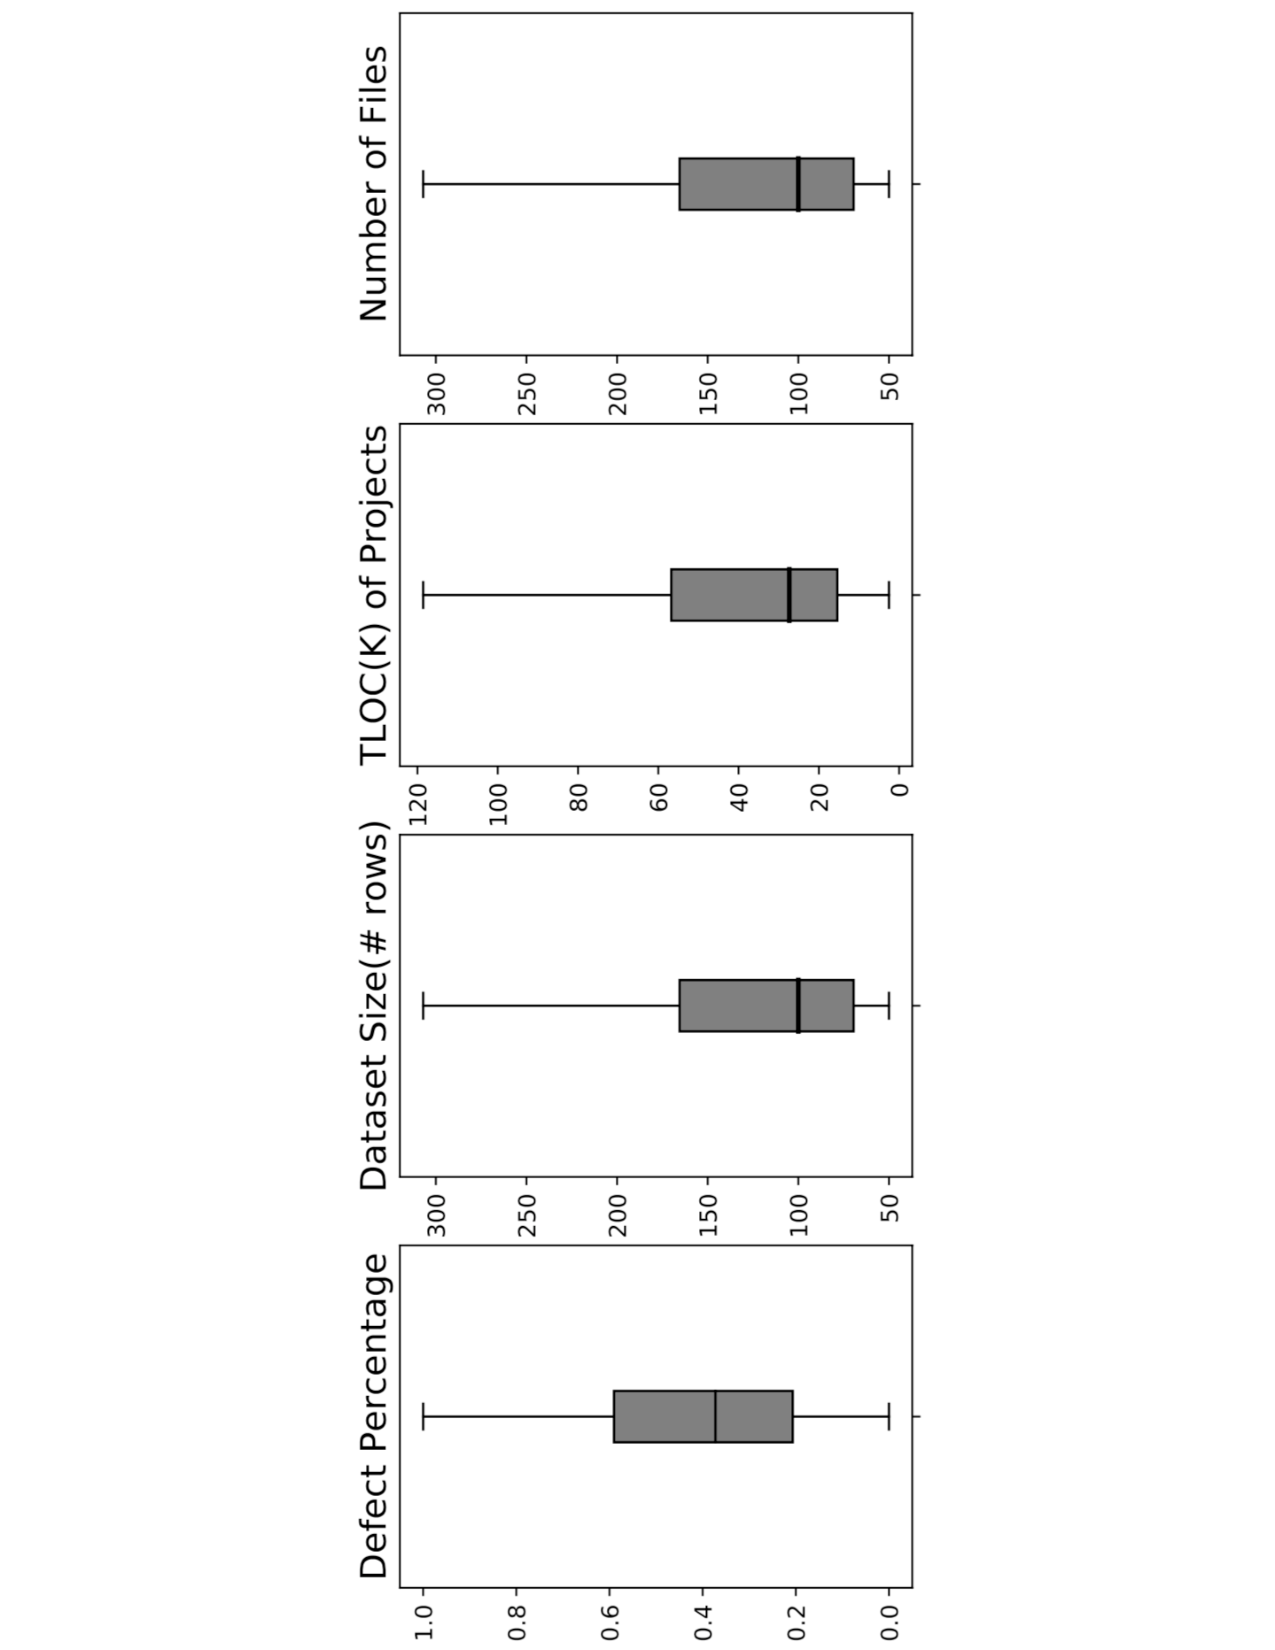
\includegraphics[width=.8\linewidth]{figs/meta.pdf}
    \caption{Distribution of projects depending on Defect Percentage, Data set Size, Lines of Code and Number of Files.}
    \label{fig:meta}
\end{figure*}


Understand is a widely used tool in software analytics~\cite{Zhang16aa,gizas2012comparative,fontana2011experience,orru2015curated,pattison2008talk,malloy2002testing}.
 The advantage of using this tool is that much of the tooling needed for this kind of large scale analysis is already available. On the other hand, it also means that we can only reason about the features that Understand can report-- which could be  a threat to the validity of the conclusions reached. As shown below, the Table~\ref{tbl:metric} metrics were shown to be effective for our task. Nevertheless, in future work, this study needs to be repeated whenever new tools allow for the widespread collection of different kinds of features.
 
\begin{table}[!t]
 

\scriptsize
\begin{tabular}{|p{1cm}|c|l|p{3cm}|}
\hline
\multicolumn{1}{|l|}{\textbf{Metric}}        & \multicolumn{1}{l|}{\textbf{Metric level}} & \textbf{Metric Name} &\textbf{ Metric Description}             \\ \hline
\multirow{21}{*}{Product   } & \multirow{6}{*}{File}             & LOC         & Lines of Code                  \\ \cline{3-4} 
                                  &                                   & CL          & Comment Lines                  \\ \cline{3-4} 
                                  &                                   & NSTMT       & Number of Statements           \\ \cline{3-4} 
                                  &                                   & NFUNC       & Number of Functions            \\ \cline{3-4} 
                                  &                                   & RCC         & Ratio Comments to Code         \\ \cline{3-4} 
                                  &                                   & MNL         & Max Nesting Level              \\ \cline{2-4} 
                                  & \multirow{12}{*}{Class}           & WMC         & Weighted Methods per Class     \\ \cline{3-4} 
                                  &                                   & DIT         & Depth of Inheritance Tree      \\ \cline{3-4} 
                                  &                                   & RFC         & Response For a Class           \\ \cline{3-4} 
                                  &                                   & NOC         & Number of Immediate Subclasses \\ \cline{3-4} 
                                  &                                   & CBO         & Coupling Between Objects       \\ \cline{3-4} 
                                  &                                   & LCOM        & Lack of Cohesion in Methods    \\ \cline{3-4} 
                                  &                                   & NIV         & Number of instance variables   \\ \cline{3-4} 
                                  &                                   & NIM         & Number of instance methods     \\ \cline{3-4} 
                                  &                                   & NOM         & Number of Methods              \\ \cline{3-4} 
                                  &                                   & NPBM        & Number of Public Methods       \\ \cline{3-4} 
                                  &                                   & NPM         & Number of Protected Methods    \\ \cline{3-4} 
                                  &                                   & NPRM        & Number of Private Methods      \\ \cline{2-4} 
                                  & \multirow{3}{*}{Methods}          & CC          & McCabe Cyclomatic Complexity   \\ \cline{3-4} 
                                  &                                   & FANIN       & Number of Input Data           \\ \cline{3-4} 
                                  &                                   & FANOUT      & Number of Output Data          \\ \hline
\multirow{5}{*}{Process }  & \multirow{5}{*}{File}             & NREV        & Number of revisions            \\ \cline{3-4} 
                                  &                                   & NFIX        & Number of revisions a file     \\ \cline{3-4} 
                                  &                                   & ADDED LOC    & Lines added                    \\ \cline{3-4} 
                                  &                                   & DELETED LOC  & Lines deleted                  \\ \cline{3-4} 
                                  &                                   & MODIFIED LOC & Lines modified                 \\ \hline
\end{tabular}
\caption{List of software metrics used in this study.}
\label{tbl:metric}
\end{table}
\subsection{Hierarchical Clustering}\label{sec:hc}

 After data collection, comes  the  hierarchical clustering needed for step 2.
For this purpose, we followed the
advice from the scikit.learn~\cite{scikit-learn} documentation
that recommends the  Balanced Iterative Reducing and Clustering using Hierarchies  (BIRCH) algorithm for hierarchical
clustering for large sample datasets that might
contain spurious outliers~\cite{zhang1996birch}. 
BIRCH has the ability to incrementally and dynamically cluster incoming, multi-dimensional data in an attempt to maintain  best quality clustering. BIRCH also has the ability to identify data points that are not part of the underlying pattern (so it can effectively identifying and avoid outliers). 
 Google Scholar reports that  the original  paper proposing BIRCH has been cited over 5,400 times.
For this experiment we used defaults proposed by~\cite{zhang1996birch}; a   branching factor of 20 and  the ``new cluster creation'' threshold  of  0.5.

 



\subsection{Data Mining}\label{sec:dm}
The bellwether analysis of step3 requires a working data miner. Three requirements for that learner are:
\bi
\item Since it will be called thousands of times, it must run quickly. Hence, we did not use any methods
that require  neural nets or ensembles. 
\item Since some projects have relatively few defects, before learning, 
some {\em over-sampling} is required to increase the number of defective examples in the training sets.
\item Since one of our research questions ({\bf RQ6}) asks ``what did we learn from all these projects'', we needed a learning method that generate succinct models. According, we used {\em feature selection}  to check which subset of Table~\ref{tbl:metric}
mattered the most.
\ei
According, this study used:
\bi
\item
The logistic regression learner, \respto{1-5a} {\color{blue} since it is widely used in defect prediction~\cite{ghotra2015revisiting,XXX} in software engineering domain and it is relatively fast in terms of model building time than other learners such as Support Vector Machine, Random Forest, Artificial Neural Nets etc. tested on defect prediction.~\cite{ghotra2015revisiting};}
\item
The SMOTE class imbalance correction algorithm\footnote{  The SMOTE Synthetic Minority Over-Sampling Technique algorithms sub-samples the majority class (i.e., deletes examples) while over-sampling the minority class until all classes have the same frequency. To over-sample, new examples are synthesized extrapolating between known examples (of the minority class) and its $k$ nearest neighbors.}~\cite{Chawla2002}, \respto{1-5b} {\color{blue} since many of the projects have relatively very few or large number of defects. A model build on project with such skewed class distribution can result in a biased model towards the majority class (Such models can either have low recall or high recall with high pf). Thus we run SMOTE on the training data\footnote{While it is useful
  to artificially boost the number of target examples
in the training data~\cite{Chawla2002,Pelayo2007,mensah2017investigating}, it is a methodological error to also change the distributions in   the test data~\cite{agrawal17}. Hence, for our work,
we take care to {\em only} resample the training data.} to artificially boost the number of target examples in the training data and achieving balanced recall and pf for the minority class test examples};
\item
Hall's
CFS feature selector~\cite{hall1999correlation}\footnote{CFS  is based on the heuristic
that ``good feature subsets contain features highly correlated with the classification, yet uncorrelated to each other''. Using this heuristic,
CFS performs a best-first search  to discover interesting sets of features.
Each subset is  scored via
$\mathit{merit}_s = kr_{\mathit{cf}}/\sqrt{k+k(k-1)r_{\mathit{ff}}}$
where
$\mathit{merit}_s$ is the value of some subset $s$ of the
features containing $k$ features; 
$r_{\mathit{cf}}$ is a score describing the connection of that feature
set to the class;
and $r_{\mathit{ff}}$ is the mean score of the feature to feature
connection between the items in $s$.
Note that for this to be maximal, $r_{\mathit{cf}}$  must be large
and $r_{\mathit{ff}}$ must be small. That is, features have to connect more to the class than each other.}, \respto{1-5c} {\color{blue} to identify features which are highly correlated with the classification, yet uncorrelated to each other. The features which are  highly correlated with each other will not add more information while making classification, while the features which are uncorrelated towards the classification also not add more information while making classification. The CFS algorithm incrementally picks one feature at a time which adds the most information towards the classification at a given step and stops when there is no more improvement in the score (see footnote 4). }
\ei
We selected  use these tools
since   in the domain of software analytics,
the use of LR (logistic regression) and SMOTE
is endorsed by recent ICSE papers~\cite{Rahman:2013,ghotra2015revisiting,agrawal17}.
As to CFS, we found that without it, our recalls were very low and we could not identify which metrics mattered the most.
Also,   extensive studies have found that CFS more useful than many other feature subset selection methods such as  PCA or InfoGain or RELIEF\respto{1-5e} {\color{blue}~\cite{hall1999correlation,challagulla2008empirical,arar2015software,lee2016developer,rodriguez2007attribute,gao2015combining,hosni2017investigating}. }






\subsection{Select the Best Model}\label{sec:best}
% As discussed below, the defect models assessed in these experiments 

To find the bellwether, our method must compare many models and select the best one based on the goals important for that task. 

In such   {\em multi-objective} problems, one model is better than another if it
 satisfies a ``domination predicate''.
 We use the Zitler indicator dominance
 predictor~\cite{zit02} to select our bellwether (since this is known to select better models
 for 5-goal optimization~\cite{Sayyad:2013,Sayyad:2013:SPL}).
This predicate favors model
  $y$ over $x$  model if $x$ ``losses'' most:
\begin{equation}\label{eq:cdom}
\begin{array}{rcl}
\textit{worse}(x,y)& =& \textit{loss}(x,y) > \textit{loss}(y,x)\\
\textit{loss}(x,y)& = &\sum_j^n -e^{\Delta(j,x,y,n)}/n\\
\Delta(j,x,y,n) & = & w_j(o_{j,x}  - o_{j,y})/n
\end{array}
\end{equation}
where  ``$n$'' is the number of objectives (for us, $n=5$) and $w_j\in \{-1,1\}$ depending on whether
we seek to maximize goal $x_j$.  

An alternative to the Zitler indicator is    `boolean domination '' that says one thing is better than another it if it no worse on any criteria and better on at least one criteria. We prefer Equation~\ref{eq:cdom} to boolean domination since we have a   3-goal optimization problem and it it is known that boolean domination often  fails for 2 or more goals~\cite{Wagner:2007,Sayyad:2013}. 
 
As discussed above, model performance can be scored and the best model can be chosen by researchers based on their choice of metrics. In this experiment we score model performance according to three goals i.e. recall, precision, pf, and chose the best model where we can:
\bi
\item
\respto{1-5f} {\color{blue}Maximize
recall\footnote{{\color{blue}Recall is the ratio between predicted actual target class examples vs all target class examples. In other words recall = $ \frac{TP}{TP+FN} $, which means in an ideal scenario where we identify all the actual target class as target class without missing the recall will be one. Thus to make a good predictor we need to maximize the recall}} and precision\footnote{{\color{blue}Precision is the ratio between predicted actual target class examples vs all predicted target class examples. In other words precision = $ \frac{TP}{TP+FP} $, so in an ideal scenario where we identify all the actual target class as target class without predicting any non-target class as target class the precision will be one. Thus to make a good predictor we need to maximize the precision as well}} 
%and popt(20)\footnote{{\color{blue}popt(20) is a cost sensitive productivity based metric, which represents the percentage of total defect identified by reading 20\% of the code. This means more defects we can identify by reading only 20\% of the code is better for the developers to localize and fix the defects.}}
};
\item
\respto{1-5f} {\color{blue} While minimizing  false alarms\footnote{{\color{blue}false alarms (pf) is the ratio between non-target class identified as target class and total number of actual non-target class. IN other words false alarm = $ \frac{FP}{FP+TN} $, so in an ideal scenario FP should be zero, thus not identifying and non-defective class as defective and effectively making false alarm as zero.}}
%and ifa\_auc\footnote{{\color{blue}Need to describe ifa auc XXXX.}}
.}
\ei
(For definitions and details for these criteria, and why we selected them, see \S\ref{sec:Measures}.)

% In such   {\em multi-objective} problems, one model is better than another if it
%  satisfies a ``domination predicate''.
%  We use the Zitler indicator dominance
%  predictor~\cite{zit02} to select our bellwether (since this is known to select better models
%  for 5-goal optimization~\cite{Sayyad:2013,Sayyad:2013:SPL}).
% This predicate favors model
%   $y$ over $x$  model if $x$ ``losses'' most:
% \begin{equation}\label{eq:cdom}
% \begin{array}{rcl}
% \textit{worse}(x,y)& =& \textit{loss}(x,y) > \textit{loss}(y,x)\\
% \textit{loss}(x,y)& = &\sum_j^n -e^{\Delta(j,x,y,n)}/n\\
% \Delta(j,x,y,n) & = & w_j(o_{j,x}  - o_{j,y})/n
% \end{array}
% \end{equation}
% where  ``$n$'' is the number of objectives (for us, $n=5$) and $w_j\in \{-1,1\}$ depending on whether
% we seek to maximize goal $x_j$.  

% An alternative to the Zitler indicator is    `boolean domination ''
%  that says one thing is better than another it if it no worse on any criteria and better on at least one criteria. We prefer Equation~\ref{eq:cdom} to boolean domination since we
%  have a   5-goal optimization problem and it it is known that boolean domination often  fails for 3 or more goals~\cite{Wagner:2007,Sayyad:2013}. 
 

% The above equation is actually Pearson's correlation  where
% all variables have been standardized.  To be applied
% for discrete class learning (as done by KDP and this paper),
% Hall et al. employ the Fayyad Irani discretizer~\cite{FayIra93Multi} then apply the following
% entropy-based measure to infer $r$ (the degree of associations
% between  discrete sets $X$ and $Y$):

% \begin{equation}\label{eq:cfs}
% r_{\mathit{xy}}=2\times \left[ \frac{H(x) + H(y) - H(x,y)}{H(y)+H(x)} \right]
% \end{equation}
% where $H$ is the standard information gain measure used in 
% decision tree learning.
% \lstset{language=Python}
% \lstset{frame=lines} 
% \lstset{label={lst:code_direct}}
% \lstset{basicstyle=\footnotesize}
% \begin{center}\begin{minipage}{2.5in}\begin{lstlisting}
% def CFS(data):
%   features = []
%   score = -1
%   while True:
%     best = None
%     for feature in range(data.features):
%       features += [feature]
%       tmp = merit( data, features) # see above equation
%       if tmp > score:
%         score = tmp
%         bests = features
%       features.pop()
%     features += bests
%     if not improve(score): break
%   return features
% \end{lstlisting}
% \end{minipage}\end{center}
% \end{figure}


%  This algorithm works is  works in 6 stages.

%     (1) \textbf{Feature Extraction:} In this stage the whole dataset is used to extract features from each project. This is done using the FSS algorithm as shown in~\ref{subsec:FSS}. Here each project is sent to the FSS and the FSS returns most suitable features for building models, we do this for every project and that information as a vector (i.e. a vector or length equal to total number of features, where 0,1 represents a feature being absent,selected) that represents each project. By performing this we have a vector representation of each project in the dataset. GENERAL uses this information to create the hierarchical clusters to find the communities. We perceive this is a good representation of community, as in this work we try to find community which has similar information distribution according to the attributes. Thus 2 projects with similar features selected have much higher chance of building similar models.
    
%     (2) \textbf{Cluster Creation:} After the feature extraction has been done, the data is sent to a modified BIRCH algorithm. The algorithm requires a branching factor (i.e. Maximum number of CF sub-clusters in each node) and threshold value (i.e. when to form a new cluster based on radius). For this experiment we have set the branching factor as 20 and threshold value as 0.5. Using this version of BIRCH algorithm we build the hierarchical cluster, while storing all necessary details about the cluster like parent-child node, data points, level information, etc. This stage returns a Clustering Feature Tree (CF Tree) with all this information, which is passed to the next phase of experiment. 
    
%     (3) \textbf{Bellwether selection phase 1:} The CF Tree from the last phase is passed to the hierarchical bellwether. In this phase we use \textit{bellwether method} to identify bellwether at the leaf level. Using the CF Tree, we identify the clusters at the leaf level where each cluster represents the smallest community produced by the BIRCH algorithm in the last phase. Here we use the default ``Bellwether'' to perform a $ N*(N-1) $ comparison at each cluster. Here we select each project in the cluster one by one as a source dataset for transfer learning apply SMOTE as mentioned in sec~\ref{subsec:SMOTE} to handle any data imbalance and then use the FSS algorithm to get rid of any unnecessary attributes as mentioned in sec~\ref{subsec:FSS}. This informative and balanced dataset is used to build a LR model as mentioned in sec~\ref{subsec:LR} and we measure the performance of all other projects in the community (cluster). The performance measures that are used are mentioned in sec~\ref{sec:Measures}. To find the bellwether in each community we use cdom function to find the best source dataset among each cluster considering all performance measures. This phase returns a bellwether for each cluster at the leaf level of the CF Tree.
    
%     (4) \textbf{Bellwether promotion:} In this phase of the algorithm is an iterative process, here we receive the selected bellwethers from the child clusters of each cluster in the level. This is called the bellwether promotion. Here each parent cluster instead of being represented by all projects within them, they are represented by only the bellwethers in them.  
    
%     (5) \textbf{Bellwether selection phase 2:} In this phase instead of finding a bellwether for each cluster at the level by performing a $ N*(N-1) $ comparison, we select the projects which represented as bellwether at the child nodes and then try to find a bellwether among them. So at each cluster at the level we perform a $ M*(M-1) $ comparison at each cluster where M is the selected bellwether from child clusters. This creates an order of magnitude faster \textbf{bellwether method}. This is again an iterative process, and the end of all the iterations, we will have a bellwether at each cluster at every level. 
    
%     (6) \textbf{Bellwether Prediction:} This is the transfer learning phase, when a new project is evaluated, we will use the FSS algorithm to get its features, then use the feature vectors to identify which cluster it belongs and use that cluster's bellwether as the transfer learning model.


\section{Experimental Methods}
\label{sec:Data Collection}

\begin{figure*}[!t]
    \centering
    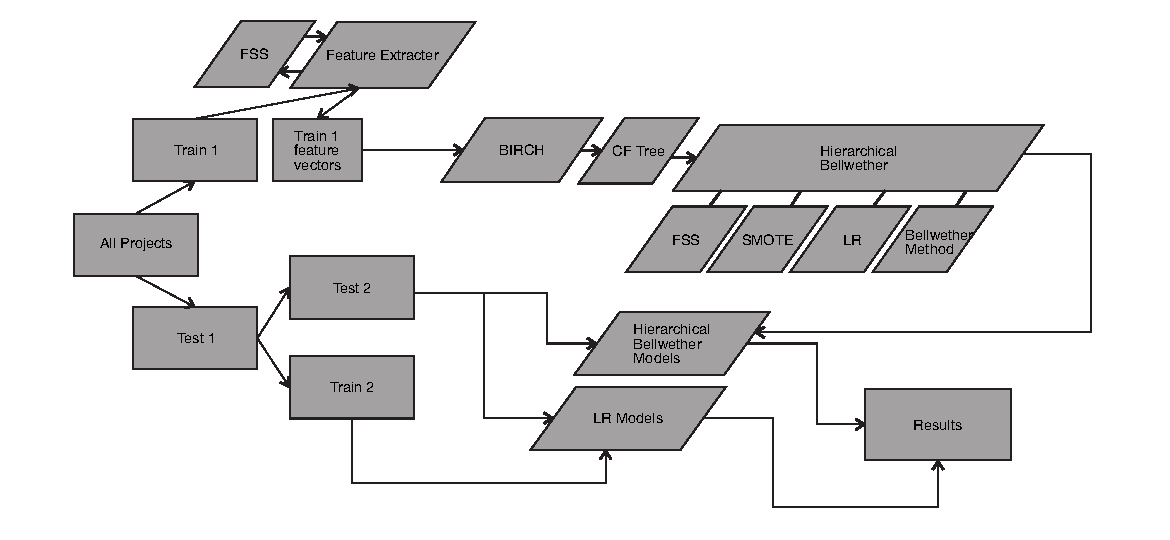
\includegraphics[width=\linewidth]{figs/General.pdf}
    \caption{ Experimental rig for this paper.  In this rig, 
      bellwethers are
    learned and tested on {\em separate } projects. Within the test set (denoted ``test1``, above),
    the data is further divided into ``train2, test2``. To assess the bellwether found from ``train1`` against local learning, data from each project is divided into ``train2,test2``
    then (a)~local
    models are learned from   ``train2``; after which time,
    (b)~the local models from ``train2'' and the bellwether model from ``train1``
    are both applied to the same data from ``test2``.
    Note that this process is repeated 20 times, with different random number seeds, to generate 20 different sets of ``train1, train2, test2``.
    }
    \label{fig:GENERAL}
\end{figure*}

\subsection{Data Collection}
\label{sec:data}

To perform our experiments we choose to work with defect prediction datasets. We use 
the data collected by Zhang et al.~\cite{zhang15}.
This data has the features of Table~\ref{tbl:metric}.
Originally, this data  was collected by Mockus et al.~\cite{mockus2009amassing} from SourceForge and GoogleCode. The dataset contains the full history of about 154,000 projects that are hosted on SourceForge and 81,000 projects that are hosted on GoogleCode to the date they were collected. In the original dataset each file contained the revision history and commit logs linked using a unique identifier. Although there were 235K,000 projects in the original database, many of there are
trivially small or are about  non-software development projects. Zhang et al. cleaned the dataset using the following    criteria:


\bi
  \item \textbf{Avoid projects with a small number of commits:} Zhang et al. removed any projects with less than 32 commits (which is the 25 \% quantile of the number of commits as the threshold). 
 
    
    \item \textbf{Avoid projects with lifespan less than one year:} Zhang et al. filtered out any  projects with a lifespan less than one year.  
    
    \item \textbf{Avoid projects with limited defect data:} Zhang et al. in their study counted the number of fix-inducing and non-fixing commits from a one-year period and removed any projects with 75 \% quantile of the number of fix-inducing and non-fixing commits.  
    
    \item \textbf{Avoid projects without fix-inducing commits:} Zhang et al. filtered out projects that have no fix-inducing commits during six months as abnormal projects, as projects in defect prediction studies need to contain both defective and non-defective commits.
\ei
On top of that, we also applied two more filters:
\bi
    \item \textbf{Use mainstream programming Languages:} the tool
    we used (Understand~\cite{visualize}) only supported     mainstream languages in widespread
    industrial use; specifically: object-oriented languages with file extension i.e *.c, *.cpp, *.cxx, *.cc, *.cs, *.java, and *.pas.
    
    \item \textbf{Avoid projects with less than 50 rows:} We removed any project with less than 50 rows as they are too small to build a meaningful predictor. 
       \item \textbf{Avoid projects with too few errors:}
    We pruned  projects which did not  have enough fix-inducing vs non-fixing data points to create a stratified k=5 fold cross-validation/% an 
    
\ei
These filters resulted in a training set of   697 projects\footnote{\href{http://tiny.cc/bellwether_data}{http://tiny.cc/bellwether\_data}}. Fig~\ref{fig:meta} and fig~\ref{fig:lang_projects} shows the Distribution of projects depending on defect percentage, data set size, lines of code, number of files and project languages to confirm the projects selected comes from wide verity and representative of a software community. 
From these selected projects, the data was labeled using issue tracking system and commit messages. If a project used issue tracking system for maintaining issue/defect history the data was labeled using that. Like  Zhang et al., we found that nearly half  of the projects did not use an issue tracking system. For these projects, labels were created analyzing commit messages by tagging them as fix-inducing commit if commit message matches the following regular expression

\begin{center}
\textit{(bug $\mid$ fix $\mid$ error $\mid$ issue $\mid$ crash $\mid$ problem $\mid$ fail $\mid$ defect $\mid$ patch)}
\end{center}
 




\subsection{Experimental Setup}
\label{sec:Experimental}


\fig{GENERAL} illustrates our experimental rig. 
 The following process was repeated 20 times, with different random seeds used each time.
 \bi
 \item
 Projects were divided
 randomly into train\_1 and test\_1 as a 90:10 split.
 \item
 The projects in train\_1 were used to find the bellwether .
 \item
 Each   project in test\_1 was  then divide into train\_2 and test\_2 (using a 2:1 split).
 \item
 LR and feature selection and SMOTE were then used
 to build two models: one from the train\_1 bellwether and one from the train\_2
 data.
 \item
 Both models were then applied to the test\_2 data.
 \ei
 




% \begin{figure}[!t]
%     \centering
%     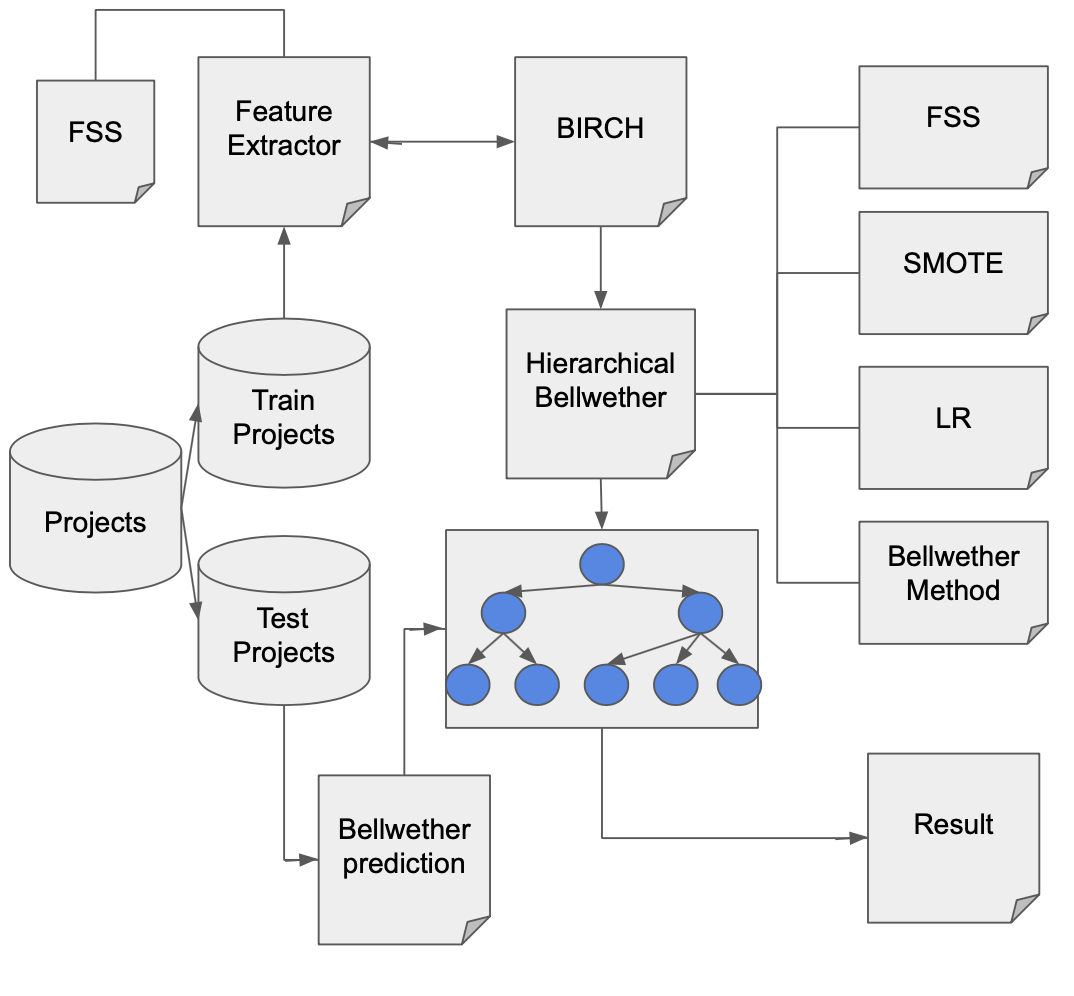
\includegraphics[width=\linewidth]{figs/BUBBLE.png}
%     \caption{GENERAL algorithm.}
%     \label{fig:GENERAL}
% \end{figure}

% In this study we try to establish the presence of generality in SE datasets. We do this by analyzing the presence of bellwether incrementally by adding more and more projects and how the bellwether's predictive power changes. In this case to show the presence of generality in SE datasets the predictive power of the bellwether should look like the \textcolor{ao(english)}{GREEN} in figure~\ref{fig:predictive_power}, that is the predictive power of bellwether should increase or remains same, if our results look like the \textcolor{red}{RED} curve, that will show absence of generality in SE datasets.

% In order to achieve this, we try to explore the \textit{bellwether effect} as mentioned in ~\ref{sec:related}. We know the default \textit{bellwether method} is very expensive ($ O(N^2) $). Thus in this paper we proposes an alternative transfer learning method (GENERAL), that explores \textit{bellwether effect} by exploring an order of magnitude faster \textit{bellwether method}. Our approach has three key components:

% \bi

%     \item A feature extractor to find a representation of each project, which will be used for clustering the projects. 
    
%     \item A hierarchical clustering model to use the features extracted from previous step to build the hierarchical cluster.
    
%     \item A transfer learning model to identify bellwether in the hierarchical cluster.

% \ei

% GENERAL employs a few different algorithms to complete and compose it's 4 different components - 

% \subsubsection{\textbf{Feature Subset Selection (FSS):}}
% \label{subsec:FSS}
% To extract features from each dataset, we use a feature selector algorithm called Feature Subset Selection(FSS)~\cite{hall1999correlation,hall1997feature}. Which is a process of identifying and removing as much irrelevant and redundant information as possible. This is achieved using a correlation based feature evolution strategy to evaluate importance of an attribute and a best first search strategy with backtracking that moves through the search space by making local changes to the current feature subset. Here if the path being explored begins to look less promising, the best first search can back-track to a more promising previous subset and continue the search from there. Given enough time, a best first search will explore the entire search space, so it uses a stopping criterion (i.e. no improvement for five consecutive attributes).

% {\small 
% \begin{figure}[]
%     \small 
%     \inputminted[numbersep=2pt, linenos=true, fontsize=\small]{python}{pseudocode/cfs.py}
%     \vspace{-0.2cm}
%     \caption{Pseudo-code of Feature Subset Selection}
%     \label{fig:GAP_pseudocode} 
%     \vspace{-0.3cm}
% \end{figure}
% } 

 
\subsection{Learners}\label{mylearners}

In this study, we applied the follow learners:

%

\textbf{Self:} (a.k.a. local learning). This  is the standard method used in software analytics~\cite{menzies2013software,zhang2013software}.
In this approach, the local project data is divided into a 90\% training set (which we call  train\_2)
and a 10\% test set (which we call test\_2). After that, some some learner builds a model from the training data
(using the methods of \S\ref{sec:Experimental}),
which is then assessed on the test data.

As we shall see, this approach produces competent defect predictors.
Recalling
the motivation of this paper: we do not
seek   better predictor that is (say) more accurate
than {\bf self}.
That is, hierarchical bellwethers can be recommended even if they {\em 
perform  no better  than {\bf self}}. Rather:
\bi
\item
As listed
in the motivations of
\S\ref{sec:Motivation}, we seek ways to make conclusions
across a wide number of projects. 
\item
That is, our goal is to test if hierarchical bellwethers
can quickly  find a  small set of {\em adequate conclusions}
that hold across a large space 
of projects. 
\ei
So, here, by ``adequate'', we mean conclusions
that perform no worse than those found by other methods.

\textbf{ZeroR:} 
In his textbook on ``Empirical AI", Cohen~\cite{Cohen:1995} recommends base-lining new methods against some simpler approach.
For that purpose, we use {\bf ZeroR} learner. This learner assigns labels every test instance according to
the majority class of the training data. Note that if anything we do performs worse that ZeroR, then there is no
point to any of the learning technology explored in this paper.  

 
\textbf{Global:}  Another baseline, against which we compare our methods
is a {\bf Global} learner build using all the data   train\_1.
Note that, if this learner performs best, then this  would  mean that we could replace GENERAL with a much simpler system.


\textbf{Bellwether0:} This learner is the  $O(N^2)$ bellwether method  proposed by Krishna et al.~\cite{krishna16a}.
What will we show is that GENERAL does better than {\bf Bellwether0} is three ways:
(a) GENERAL is inherently more scalable; (b) GENERAL is (much) faster; and (c) GENERAL produced better predictions.
That is, our new GENERAL method is a significant improvement over the prior state-of-the-art.


\textbf{GENERAL\_level2:}  GENERAL finds bellwethers at various levels of the BIRCH cluster tree.  GENERAL\_level2 results show the performance of the model learned from the bellwether found in the leaves of the  BIRCH cluster tree.
That is these results come from  a bellwether generated from 15 to 30 projects.  
For this process:
\bi
\item
First, we tag each leaf cluster with its associated bellwether;
\item
Second, we use the test procedure built into BIRCH; i.e. a test case is presented to the root
of the cluster tree and BIRCH returns its {\em relevant  leaf};
i.e. the cluster closest to that test case.
\item
We then apply the bellwether tagged at that leaf.
\ei
\textbf{GENERAL\_level1:}  GENERAL\_level1 results show the performance of the model learned from the bellwether found between the root and   the leaves of the  BIRCH cluster tree. In practice, BIRCH divides our data only twice
so there is only one GENERAL\_level1  between root and leaves. For this process,
we use the same procedure as GENERAL\_level2 but this time, we use the bellwether tagged in the {\em parent}
cluster of the relevant leaf. Note that these level1 results come from an analysis of between 50 to 200  projects
(depneding on the shape of the cluster tree genrated via BIRCH). 



\textbf{GENERAL\_level0:}  
In the following,  the  GENERAL\_level0 results show the performance of the model learned from the bellwether found at the root of the BIRCH cluster tree. Note that these results come from an analysis of over 600 projects. 

 
\subsection{Statistical Tests}
\label{stats}\label{eval}

When comparing the results different models in this study, we used a statistical significance test and an effect size test. Significance test is useful for detecting if two populations
differ merely by random noise. Also, effect sizes are useful for checking that two populations differ by more than just a trivial amount. For the significance test,  we use the Scott-Knott procedure  recommended at TSE'13~\cite{mittas2013ranking} and ICSE'15~\cite{ghotra2015revisiting}. This technique recursively bi-clusters a sorted set of numbers. If any two clusters are statistically indistinguishable, Scott-Knott reports them both as one group. Scott-Knott first looks for a break in the sequence that maximizes the expected values in the difference in the means before and after the break. More specifically,  it  splits $l$ values into sub-lists $m$ and $n$ in order to maximize the expected value of differences  in the observed performances before and after divisions. For e.g., lists $l,m$ and $n$ of size $ls,ms$ and $ns$ where $l=m\cup n$, Scott-Knott divides the sequence at the break that maximizes:
\begin{equation}
    E(\Delta)=\frac{ms}{ls}\times abs(m.\mu - l.\mu)^2  + \frac{ns}{ls}\times abs(n.\mu - l.\mu)^2
\end{equation}
Scott-Knott then applies some statistical hypothesis test $H$ to check if $m$ and $n$ are significantly different. If so, Scott-Knott then recurses on each division. For this study, our hypothesis test $H$ was a conjunction of the A12 effect size test (endorsed by \cite{arcuri2011practical})  and non-parametric bootstrap sampling \cite{efron94}, i.e., our Scott-Knott divided the data if {\em both} bootstrapping and an effect size test agreed that the division was statistically significant (90\% confidence) and not a ``small'' effect ($A12 \ge 0.6$).



\subsection{Performance Measures}
\label{sec:Measures}

In this section, we introduce the following 5 evaluation measures used in this study to evaluate the performance of machine learning models. Suppose we have a dataset with M changes and N defects. After inspecting 20\% LOC, we inspected $m$ changes and found $n$ defects. Also, when we find the first defective change, we have inspected k changes. Using
this data, we can define 5 evaluation measures  as follows:

(1) \textbf{Recall:} This is the proportion of inspected defective changes among all the actual defective changes; i.e. $n/N$.
Recall is used in  many previous studies~\cite{kamei2012large,yang2016effort,yang2017tlel,xia2016collective,yang2015deep}.  

(2) \textbf{Precision:} This is the proportion of inspected defective changes among all the inspected changes; i.e. $n/m$. A low Precision indicates that developers would encounter more false alarms, which may have negative impact on developers' confidence on the prediction model.  

(3) \textbf{pf:} This is the proportion of all suggested defective changes which are not actual defective changes among all the suggested defective changes. A high {\em pf} suggests developers will encounter more false alarms which may have negative impact on developers' confidence in the prediction model.

(4) \textbf{popt20:} This is the proportion number of suggested defective changes among all suggested defective changes, when when 20\% LOC modified by all changes are inspected. 
A high {\em popt20} values mean that developers can find most bugs in a small percent of the code.
To compute Popt20, we divided the test set into the modules predicted to be faulty (set1)
and predicted to be bug-free (set2). Each set was then sorted in ascending order by lines 
of code.  We then ran down set1, then set2, till 20\% of the total lines of code
were reached-- at which point {\em popt20} is the percent of buggy modules seen up to that point.

(5) \textbf{ifa\_auc:} Number of  initial false alarms encountered before we find the first defect. Inspired by previous studies on fault localization~\cite{parnin2011automated,kochhar2016practitioners,xia2016automated}, we caution that if the top-k changes recommended by the model are all false alarms, developers would be frustrated and are not likely to continue inspecting the other changes. For example, Parnin and Orso ~\cite{parnin2011automated} found that developers would stop inspecting suspicious statements, and turn back to traditional debugging, if they could not get promising results within the first few statements they inspect. Using the nomenclature reported
about {\em Ifa$=k$}.  In this study we use a modified version of {\em ifa} called ifa\_auc, which calculates {\em ifa} based on efforts spent on inspecting the code. We use gradually increment the efforts spent by increasing the total LOC inspected and calculate ifa on each iteration to get the area under the curve (auc), here the x-axis is the percentage of effort spent on inspection and y-axis is {\em ifa}.


\section{Results}
\label{sec:results}

\subsection*{RQ1: How slow is conventional bellwether method? }
\label{sec:rq3}

\subsection*{RQ2: How  fast  is  new  bellwether  method  aka  GENERAL?}
\label{sec:rq3}


\subsection*{RQ3: Can hierarchical clustering tame the complexity of bellwether-based reasoning?}
\label{sec:rq3}

% In the literature, we saw most of the previous studies have shown bellwether effect with very small datasets. In order to use bellwether to prove presence of generality in SE domain datasets, we first have to showcase the bellwether method suggested by Krishna et al. in their experiment works for large datasets. We use our defect prediction dataset with 697 projects for this purpose. 

% We divide the dataset in train\_1 and test\_1 set and then performed a $ N*(N-1) $ comparison on all the projects in train\_1 set to find a bellwether, and then dividing each project in test\_1 set into train\_2 and test\_2 using a train\_test split. We use the train\_2 to train a LR model and test on test\_2 which is represented as \textit{self} in the figures. Similarly we use the bellwether project from train\_1 to train a LR model and test it on test\_2 which is represented as \textit{bellwether0}. We use statistical tests mentioned in section~\ref{stats} to compare the performance of \textit{self} vs \textit{bellwether0} for all the performance measures mentioned in section~\ref{sec:Measures}, which is shown 
 
\fig{cost} showed that, theoretically,
GENERAL is an inherently faster approach than traditional bellwether methods.
To test that theoretical
conclusion,
we ran the rig of \fig{GENERAL} on
an four core machine running at 2.3GHz with 8GB of RAM. 



\begin{figure}[!b]
    \centering
    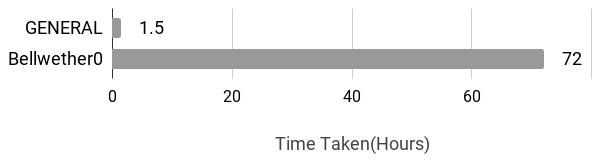
\includegraphics[width=\linewidth]{figs/Time.png}
    \caption{Mean runtime for for one run of standard bellwether and GENERAL.}
    \label{fig:time}
\end{figure}


\fig{time} shows the mean runtimes for one run of GENERAL versus traditional bellwether. For certification purposes, this had to be repeated 20 times. In that certification run:
\bi
\item
The $O(N^2)$ analysis of the traditional {\em bellwether0} approach needed 60 days of CPU time.
\item 
The $O(m*(N/m)^2)$ analysis
of GENERAL needed 30  hours. That is, in empirical
 result consistent with the theoretical predictions of \fig{cost}, GENERAL runs much faster than traditional bellwether.
\item All the other methods required
another 6 hours of computation. 
\ei
If we were merely seeking conclusions from one project, then we would recommend ignoring bellwethers
and just use results from each project. That said, we still endorse bellwether method since  we seek
lessons that hold across many projects.

In summary, based on these results, we conclude that:


\begin{RQ}{Theoretically and empirically, the  hierarchical reasoning on GENERAL performs much faster than standard bellwether methods.}
\end{RQ}





%%%%%%%%%%%%%%%%%%%%%%%%%%%%%%%%%%%%%%%%%%%%%%%%%%%%%%%%%%%
%%%%%%%%%%%%%%%%%%%%%%%Latex Table%%%%%%%%%%%%%%%%%%%%%%%%%
\begin{figure}[!b]
{\scriptsize
{\scriptsize \begin{tabular}{p{.1cm}lp{1.5cm}rrc}
\arrayrulecolor{darkgray}
\rowcolor[gray]{.9}  & rank & treatment & mean & sd & \\
 \multirow{5}{*}{\rotatebox[origin=c]{90}{Recall}} 
  &   1 &      GENERAL\_level2 &    38 &  32 & \quart{22}{38}{32}{16} \\
  &   1 &      bellwether0 &    39 &  31 & \quart{23}{39}{31}{15} \\
  &   1 &  ZeroR &    40 &  49 & \quart{16}{40}{49}{25} \\
  &   2 &      GENERAL\_level1 &    48 &  33 & \quart{31}{48}{33}{16} \\
  &   3 &      self &    55 &  27 & \quart{41}{55}{27}{12} \\
  &   3 &      GENERAL\_level0 &    56 &  31 & \quart{42}{56}{31}{16} \\
  &   4 &      global &    78 &  40 & \quart{57}{78}{40}{20} \\ \hline
\multirow{5}{*}{\rotatebox[origin=c]{90}{Pf}} 
  &  1 &      GENERAL\_level2 &    28 &  28 & \quart{14}{28}{28}{13} \\
  &  1 &      bellwether0 &    28 &  25 & \quart{15}{28}{25}{11} \\
  &  1 &      self &    30 &  20 & \quart{20}{30}{20}{10} \\
  &  1 &      GENERAL\_level1 &    35 &  28 & \quart{21}{35}{28}{14} \\
  &  1 &      ZeroR &    39 &  49 & \quart{15}{39}{49}{25} \\
  &  2 &      GENERAL\_level0 &    47 &  31 & \quart{31}{47}{31}{15} \\
  &  3 &      global &    79 &  39 & \quart{59}{79}{39}{19} \\\hline
\multirow{5}{*}{\rotatebox[origin=c]{90}{Precision}} &   1 &      ZeroR &    21 &  30 & \quart{6}{21}{30}{15} \\
    &  2 &      global &    35 &  28 & \quart{21}{35}{28}{14} \\
    &   2 &      GENERAL\_level2 &    39 &  34 & \quart{22}{39}{34}{17} \\
    &   2 &      bellwether0 &    40 &  33 & \quart{23}{40}{33}{16} \\
    &   2 &      GENERAL\_level1 &    42 &  31 & \quart{26}{42}{31}{15} \\
    &   2 &      GENERAL\_level0 &    44 &  30 & \quart{28}{44}{30}{15} \\
    &   2 &      self &    50 &  30 & \quart{35}{50}{30}{15} \\\hline
\multirow{5}{*}{\rotatebox[origin=c]{90}{Popt20}} &   1 &      ZeroR &    13 &  16 & \quart{5}{13}{16}{8} \\
  & 2 &      GENERAL\_level2 &    26 &  22 & \quart{15}{26}{22}{11} \\
  &  2 &      global &    26 &  13 & \quart{19}{26}{13}{6} \\
  &  2 &      bellwether0 &    28 &  21 & \quart{17}{28}{21}{9} \\
  &  2 &      GENERAL\_level0 &    28 &  15 & \quart{22}{28}{15}{8} \\
  &  2 &      GENERAL\_level1 &    28 &  19 & \quart{19}{28}{19}{9} \\
  &  3 &      self &    35 &  19 & \quart{26}{35}{19}{10} \\\hline
\multirow{5}{*}{\rotatebox[origin=c]{90}{ifa\_auc}} &   1 &      ZeroR &    7 &  11 & \quart{1.12}{6.77}{11.29}{5.65} \\
  &  2 &      global &    19 &  16 & \quart{11.35}{19.38}{16.06}{8.03} \\
  &  3 &      GENERAL\_level2 &    22 &  14 & \quart{14.48}{21.59}{14.21}{7.10} \\
  &  3 &      bellwether0 &    23 &  14 & \quart{15.48}{22.56}{14.15}{7.07} \\
  &  3 &      self &    23 &  12 & \quart{17.09}{22.93}{11.68}{5.84} \\
  &  3 &      GENERAL\_level1 &    23 &  14 & \quart{16.10}{22.98}{13.74}{6.87} \\
  &  3 &      GENERAL\_level0 &    25 &  13 & \quart{17.87}{24.51}{13.27}{6.63} \\
\end{tabular}}
}
\caption{Statistical Results comparison. The ``rank`` column at left comes from
the statistical analysis methods of \S\ref{eval}. Note that for {\em pf}, and {\em ifa} rank=1 is the best rank while for all other performance measures, ranks $\in{3,4}$ are best. 
}\label{fig:Statistical}
\end{figure}

% {\small 
% \begin{figure*}[!t]
%     \centering
%     \begin{tikzpicture}[nodes={draw, circle,fill=darkgray!60}, ->,sibling distance=.7cm,minimum size=.1cm,scale=.5]
 
%     \node{627}
%         child { node {57}
%             child {node {9}} 
%             child {node {9}} 
%             child {node {7}} 
%             child {node {17}}
%             child {node {13}}}
%         child [missing]
%         child [missing]
%         child [missing]
%         child [missing]
%         child [missing]
%         child [missing]
%         child [missing]
%         child { node {127} 
%             child {node {3}} 
%             child {node {9}} 
%             child {node {19}} 
%             child {node {15}}
%             child {node {4}}
%             child {node {17}} 
%             child {node {15}} 
%             child {node {19}} 
%             child {node {11}}
%             child {node {15}}}
%         child [missing]
%         child [missing]
%         child [missing]
%         child [missing]
%         child [missing]
%         child [missing]
%         child [missing]
%         child [missing]
%         child [missing]
%         child [missing]
%         child [missing]
%         child [missing]
%         child { node {183} 
%             child {node {8}} 
%             child {node {3}} 
%             child {node {12}} 
%             child {node {16}}
%             child {node {20}}
%             child {node {18}} 
%             child {node {12}} 
%             child {node {4}} 
%             child {node {12}}
%             child {node {16}}
%             child {node {5}}
%             child {node {17}} 
%             child {node {9}} 
%             child {node {9}} 
%             child {node {10}}
%             child {node {14}}}
%         child [missing]
%         child [missing]
%         child [missing]
%         child [missing]
%         child [missing]
%         child [missing]
%         child [missing]
%         child [missing]
%         child [missing]
%         child [missing]
%         child [missing]
%         child [missing]
%         child [missing]
%         child [missing]
%         child [missing]
%         child [missing]
%         child [missing]
%         child { node {260} 
%             child {node {17}} 
%             child {node {17}} 
%             child {node {20}} 
%             child {node {14}}
%             child {node {9}}
%             child {node {13}} 
%             child {node {18}} 
%             child {node {10}} 
%             child {node {18}}
%             child {node {10}}
%             child {node {6}} 
%             child {node {15}} 
%             child {node {14}} 
%             child {node {9}}
%             child {node {10}}
%             child {node {8}} 
%             child {node {7}} 
%             child {node {13}} 
%             child {node {15}}}
%             ;
% \end{tikzpicture}
%     \caption{Example of Hierarchical Clustering for 627 projects}
%     \label{fig:example tree}
% \end{figure*}
% }
%%%%%%%%%%%%%%%%%%%%%%%End Latex Table%%%%%%%%%%%%%%%%%%%%%
%%%%%%%%%%%%%%%%%%%%%%%%%%%%%%%%%%%%%%%%%%%%%%%%%%%%%%%%%%%
\begin{figure*}[!t]
    \centering
    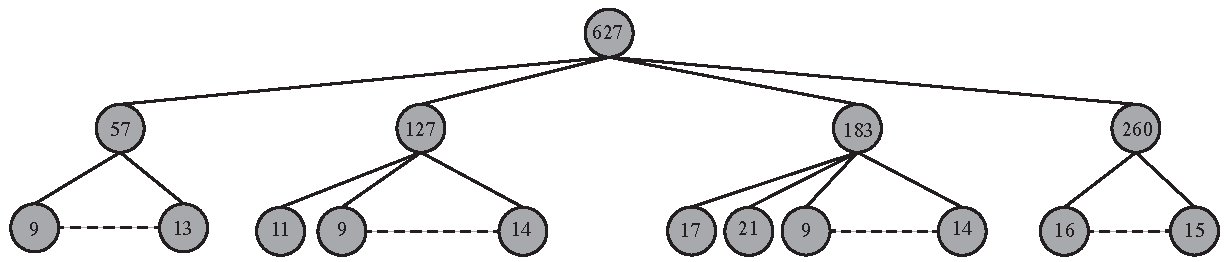
\includegraphics[width=\linewidth]{figs/bubble.pdf}
    \caption{Example of Hierarchical Clustering for 627 projects}
    \label{fig:example tree}
\end{figure*}



 

\subsection*{RQ4: Is this faster bellwether effective?}
\label{sec:rq4}

The speed improvements reported in {\bf RQ3} are only useful
of this faster method can also deliver adequate predictions
(i.e. predictions that are not worse
than those generated by other methods).

 
Figure~\ref{fig:Statistical} shows the distribution of
performance score results seen in
of \fig{GENERAL}. These results are grouped together by the ``rank'' score
of the left-hand-side column 
(and this rank was generated using the statistical methods of
\S\ref{eval}).


In these results, the {\em ifa\_auc}  and {\em precision} scores
were mostly uninformative. With the exception of {\em ZeroR},
there was very little difference in these scores.

As to {\em ZeroR}, we cannot recommend that approach.
While {\em ZeroR} 
makes few mistakes (low {\em ifa}s and low {\em pf}s), it scores badly
on   other measures (very low {\em recall}s  and {\em popt(20)}.

Similarly, we cannot recommend the    {\em global} approach.
In this approach, quality predictors are learned from   one data set that combines
data from hundreds of projects. As seen in Figure~\ref{fig:Statistical} 
that approach generates an unacceptably large false alarm rate ($pf=79\%$).

Another approach we would deprecate is the traditional bellwether approach.
By all the measures of
Figure~\ref{fig:Statistical},   the {\em bellwether0} are in the middle of the pack. That is:
\bi
\item
That approach is in no way outstanding. 
\item
So, 
compared to hierarchical bellwether,
 there is no evidence here of a performance
benefit from using  traditional bellwether.
\item
Given this lack luster performance, 
and   the {\bf RQ3} results (where traditional bellwether ran very slowly), we therefore  
deprecate the traditional bellwether approach.
 \ei
As to GENERAL vs the local learning results of {\em self}, in many ways their performance in  Figure~\ref{fig:Statistical},
is indistinguishable:
\bi
\item As mentioned above, measured in terms of {\em ifa\_auc}
and {\em precision}, there is no significant differences.
\item In terms of {\em recall} there is no statistical difference in the rank
of  local learning with {\em self} and 
  {\em GENERAL\_level0}
(a bellwether
generated from the root of a BIRCH cluster tree) and 
\item In terms of {\em pf} (false alarms), some of the GENERAL results are ranked
the same as {\em self} (and we will expand on this point, below).
\ei
Overall, we summarize the Figure~\ref{fig:Statistical} results as follows:



\begin{RQ}
{Measured in terms of predictive performance,
the effectiveness of hierarchical bellwethers
is very similar to local learning
(and these two methods are more effective
than the other options explored here). }
\end{RQ}

 
When two options have similar predictive
performance, then other criteria can be used
to select between them:
\bi
\item If the goal is to quickly generate
conclusions about one project, then we would recommend
local learning since (as seen above), local learning is five
times faster than hierarchical bellwether.
\item
But, as said at the start
of \S\ref{sec:results},
our goal is to quickly generalize across hundreds of
projects. 
\ei
 



\subsection*{RQ5: Does learning from too many projects have detrimental effect?}
\label{sec:rq5}

Returning now to \fig{predictive_power}, this
research question asks if there is such a thing
as learning from too much data.  What we will see is that
answers to this question are much more complex than the simplistic
picture of \fig{predictive_power}. While for some goals it is possible
to learn from too much data, there are other goals where it seems
more is always better.

To answer {\bf RQ5}, we first note that when GENERAL
calls the BIRCH clustering algorithm, it generates the tree
of clusters shown in  
\fig{example tree}. In that tree:
\bi
\item
The bellwether found at level 0 of the tree
(which we call {\em GENERAL\_level0}) is learned from 627 projects.
\item
The bellwethers found at level 1 of the tree
(which we call {\em GENERAL\_level1}) is learned from four sub-groups
of our projects.
\item
The bellwethers found at level 2 of the tree
(which we call {\em GENERAL\_level2}) is learned from 80
sub-sub groups of our projects.
\ei
That is, to answer {\bf RQ5} we need only compare the predictive performance
of models learned from these different levels. In that comparison,
if the level\_$(i+1)$ bellwethers generated better predictions
that the   level\_$(i)$ bellwethers, then we would conclude that it is best to learn lessons from smaller groups
of projects.

Figure~\ref{fig:Statistical} lets us
compare the performance of the bellwethers learned from different 
levels:
\bi
\item The {\em ifa} and {\em Popt20} 
and {\em precision}  results for the different levels
are all ranked the same.  Hence we say that, measured in terms of those 
measures, we cannot distinguish the performance at different levels.
\item 
As to {\em recall},   the level2,1,0 bellwether results are 
respectively ranked worst, better, best. 
\item
Slightly different results are offered in the {\em pf} false alarm results. Here,  levels2,1,0 bellwether are respectively ranked best, best, worst.
\ei
That is, these results say that:

\begin{RQ}
{Assessed in terms of {\em recall},
it is better to learn bellwethers from more data rather than less.
But assessed in terms of {\em false alarms}, 
while learning bellwethers
from many projects is useful, it is possible to learn from too much data.} 
\end{RQ}

To put that another way, the answer to ``is is possible to learn from too much data'', is ``depends on what you value'':
\bi
\item
For risk-adverse development of mission or safety critical
systems, it is best to use all data to learn the bellwether
since that finds most defects.
\item
On the other hand, for cost-adverse development of non-critical
systems (where cutting development cost
is more important than removing
bugs), then there seems to be a ``Goldilocks zone'' where
the bellwether is learned from just enough data (but not too much or too little).
\ei

% In this section, we return to 
% In RQ4, we try to answer the question if learning from too many projects detrimental effect, this question has two parts, one on predictive power, the other on making general conclusion and conclusion instability. Figure~\ref{fig:Statistical} shows the results of statistical significance and effect size tests to rank them in order for all the different methods(treatments) used in this experiment. In this figure for a performance measure two methods showing same rank means there performance is not statistically significantly different, while a different ranks mean they are different, while a smaller rank is better if the performance goal is negative (i.e. Pf), and higher rank is better in case of positive goal (i.e. Recall).

% To answer the first part of the question, if learning from too many projects have detrimental effect on predictive power of models, we compare the results of default ``bellwether method'' (a.k.a bellwether0) proposed by Krishna et al. and GENERAL(a.k.a GENERAL\_level0) method. The results of scott-knott test shows that for positive goals such as Recall the GENERAL\_level0 is significantly doing better than Bellwether0 and it is doing as good as or better for precision ans recall. While for negative goals such as ifa\_auc GENERAL\_level0 is doing as good as bellwether0. Although in case of Pf they score different ranks with GENERAL showing higher Pf then bellwether0, it is not by much. Similarly while comparing GENERAL\_level0 with global (which is learning from all the projects) shows although it achieves higher Recall, but it has very high Pf, low precision. Which answers the first part of the question that learning from too many projects do have detrimental effect on predictive power of models. 


% Now to answer the second part of the question, that is if learning from too many projects creates conclusion instability, we will look at figure~\ref{fig:FSS_compare}. Figure~\ref{fig:FSS_compare} show the distribution of attributes selected while building a ML model for defect prediction using local models(a.k.a self), the \textcolor{red}{{\bf red bars}} shows the attributes selected by the ``Bellwether Project''. Conclusion instability causes vastly different and often contradicting conclusions to be derived from a data source. This sort of instability is very prevalent in several domains of software engineering. We can see from figure~\ref{fig:FSS_compare}, when learning from local data, each model selected different sets of attributes and resulted in selecting almost all different attributes. That means there is no general conclusion can be drawn for defect prediction models by saying which attributes are important, this results in conclusion instability and that effects the trusts on those models, the insights that can be drawn from them. Which farther affects training and tool development as mentioned in sec~\ref{sec:Motivation}. From these results we can see learning from too many data can cause conclusion instability and thus affecting generality in SE domain. In Summary, we can say 



\begin{figure*}[h]
    \centering
    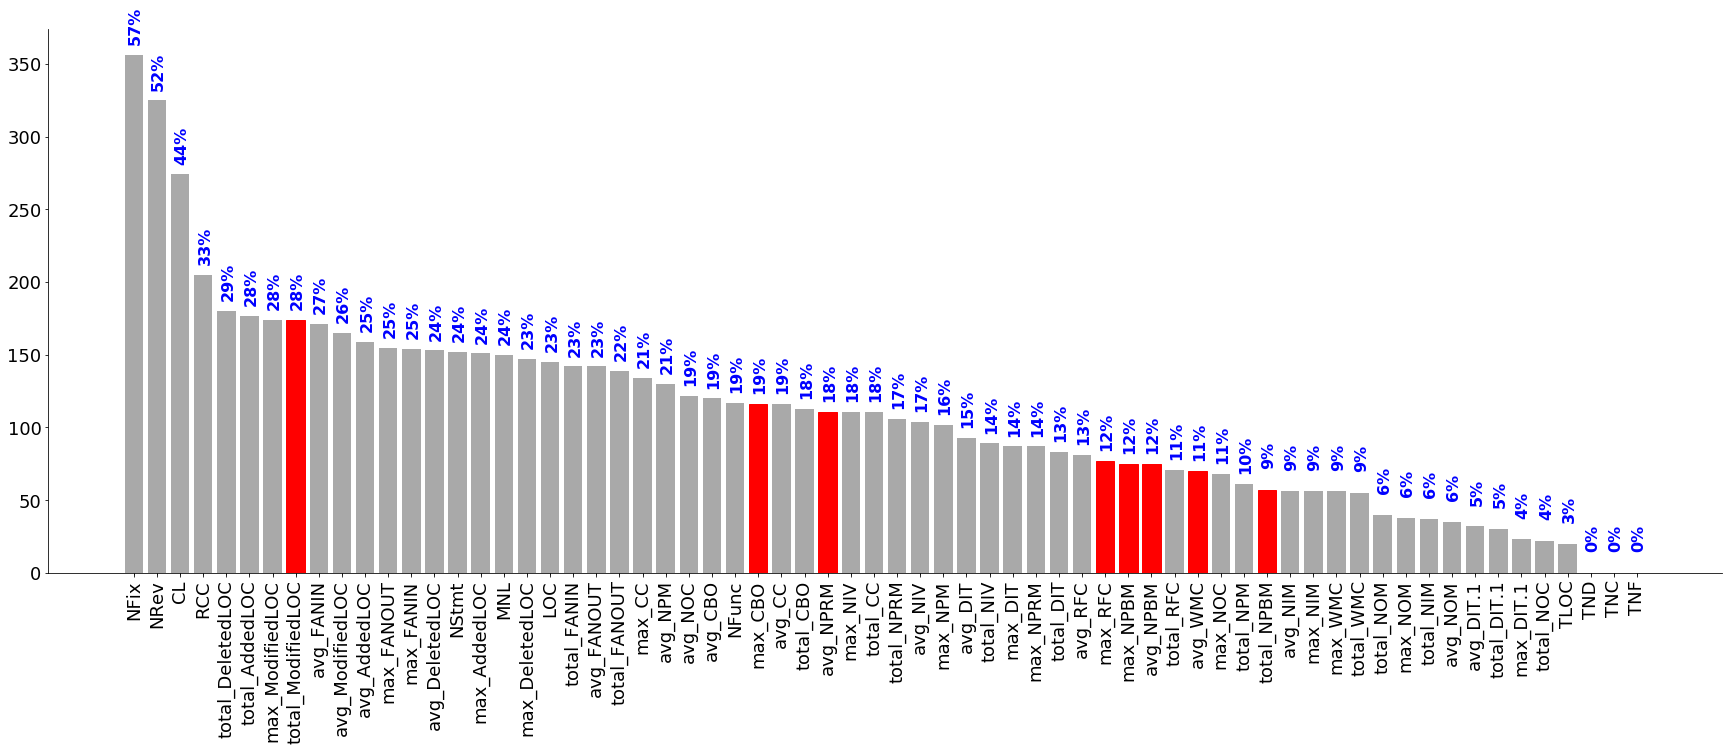
\includegraphics[width=\linewidth]{figs/FSS_compare.png}
    \caption{Distribution of features selected using self model and ``Bellwether'' model.}
    \label{fig:FSS_compare}
\end{figure*}

\subsection*{RQ6: What exactly did we learn from all those projects?}
\label{sec:rq6}

Having demonstrated that we can quickly find bellwethers
from hundreds of software projects, it is appropriate to ask
what model was learned from all that data. This is an important question for this research since if  we cannot show the lessons
learned from our 627 projects, then all the above is wasted effort.

Table~\ref{tbl:coefs}  shows the weights learned by logistic
regression after feature selection using the bellwether project
selected by {\em GENERAL\_level0}. Note that:
\bi
\item
The number of features that appear in Table~\ref{tbl:coefs}  is much smaller than the list of features shown in Table~\ref{tbl:metric}.
That is, our bellwether is reporting that only a few features
are most important for predicting software defects.
\item
Table~\ref{tbl:coefs}  is sorted by the absolute value of the weights
associated with those features. The last two features have near
zero weights; i.e. they have negligible effect.
\ei
Apart from the negligible features, all that is left are NPRM, NPNM, RFC , and CBO. As shown in Table~\ref{tbl:metric}, these features
all relate to class interface concepts; specifically: 
\bi
\item
The number of public and private methods; 
\item
The  average number of methods that respond to an incoming message; 
\item
Inter-class coupling. 
\ei
\begin{table}[!t]
\centering
\begin{tabular}{|l|l|l|l|} \hline
Rank & Attr               & coef  & Odds ratio \\ \hline
1    & avg\_NPRM          & 2.23  & 9.26      \\ \hline
2    & avg\_NPBM          & -1.31 & 0.27      \\ \hline
3    & max\_NPBM          & -1.12 & 0.33      \\ \hline
4    & max\_RFC           & 0.74  & 2.09      \\ \hline 
5    & total\_NPBM        & -0.70 & 0.50      \\ \hline
6    & max\_CBO           & -0.64 & 0.53      \\ \hline
7    & total\_ModifiedLOC & 0.10  & 1.10      \\ \hline
8    & avg\_WMC           & 0.07  & 1.07     \\ \hline
\end{tabular}

\caption{Importance of coefs on \textit{log p} from logistic regression model of ``Bellwether'' shown in Fig~\ref{fig:FSS_compare}. Here Odds ratio shows one increment in in respective variable increase in the log-odds of being defective.}\label{tbl:coefs}
\end{table}
\fig{FSS_compare} shows what might be learned with and without
the methods of this paper. Recall that the learners used in this research used feature selection and  logistic regression.
\begin{itemize}
\item  The gray bars in \fig{FSS_compare} show how often the features
of Table~\ref{tbl:metric} were selected in the models learned from
local data using {\em self}. 
\item
The red bars in \fig{FSS_compare} shows which features
used in the local models that also appeared in the model learned from the bellwether. 
  Note that only a very
small subset of the features seen in the  {\em self} models
were found useful in the bellwether model of Table~\ref{tbl:coefs}.
\end{itemize}
Just to say the obvious:
when learning
local models from very many projects, there is a wide range 
of features used in the model.
It is far easier to 
definitively learn lessons from a much smaller range
of features, such as those listed in Table~\ref{tbl:coefs}.
For example,
based on these results
we can say that for predicting defects, in this sample of  features taken from 627 projects:
\bi
\item Issues of inter-class interface are paramount;
\item While many other  issues are far less important such as file size, depth of inheritance tree, intra-method complexity, file size, revision history, and anything relating to  the other features of Table~\ref{tbl:metric}
that are not listed in Table~\ref{tbl:coefs}.
\ei
In summary:

\begin{RQ}
{The importance of many key features is not apparent at the local
project level. To fully appreciate the critical impact on defects
of class interface design,  it is necessary to conduct
a global analysis across hundreds of projects. }
\end{RQ}
To say that another way, 
\begin{quote}
{\em 
Learning from many other projects can be better than learning just from your own local project data.
}\end{quote}


\section{Threats to Validity}
\label{sec:validity}

As with any large scale empirical study, biases can affect the final
results. Therefore, any conclusions made from this work
must be considered with the following issues in mind:

(a) \textit{Evaluation Bias}: 
In  {\bf  RQ3, RQ4} and {\bf RQ5} we have shown the performance of local model, hierarchical bellwether models, default bellwether model and compared them using statistical tests on their performance to make conclusion about presence of generality in SE datasets. While those results are true, that conclusion is scoped by the evaluation metrics we used to write this paper. It is possible that, using other measurements, there may well be a difference in these different kinds of projects. This is a matter that needs to be explored in future research.  

    
(b) \textit{Construct Validity}: At various places in this report, we made engineering decisions about (e.g.) choice of machine learning models, hierarchical clustering algorithm, selecting feature vectors for each project. While those decisions were made using advice from the literature, we acknowledge that other constructs might lead to different conclusions. 

(c) \textit{External Validity}: For this study we have relied on data collected by Zhang et al.~\cite{zhang15} for their studies. The metrics collected for each project were done using an commercialized tool called ``Understand''. There is a possibility that calculation of metrics or labeling of defective vs non-defective using other tools or methods may result in different outcome. That said, the ``Understand'' is a commercialized tool which has detailed documentation about the metrics calculations and Zhang et al. has shared their scripts and process to convert the metrics to usable format and has described the approach to label defects.  

We have relied on issues marked as a `bug' or `enhancement' to count bugs or enhancements, and bug or enhancement resolution times. In Github, a bug or enhancement might not be marked in an issue but in commits. There is also a possibility that the team of that project might be using different tag identifiers for bugs and enhancements. To reduce the impact of this problem, we  did take precautionary step to (e.g.,) include various tag identifiers from Cabot et al.~\cite{cabot2015exploring}. We also took precaution to remove any pull merge requests from the commits to remove any extra contributions added to the hero programmer. 

(d) \textit{Statistical Validity}: To increase the validity of our results, we applied two statistical tests, bootstrap and the a12. Hence, anytime in this paper we reported that ``X was different from Y'' then that report was based on both an effect size and a statistical significance test.
 
(e) \textit{Sampling Bias}: Our conclusions are based on the 697 projects collected by Zhang et al.~\cite{zhang15} for their studies. It is possible that different initial projects would have lead to different conclusions. That said, this sample is very large so we have some confidence that this sample represents an interesting range of projects. As evidence of that, we note that our sampling bias is less pronounced than other ``Bellwether'' studies since we explored.
 



\section{Conclusion}
\label{sec:concl}
In this paper, we have proposed a new transfer learning  bellwether method   called GENERAL.
While GENERAL only reflects on a small percent of the projects,
its hierarchical methods find projects which yield models
whose performance is comparable to anything else we studied
in this analysis.
Using GENERAL, we have shown that issues
of class interface design were the most critical
issue within a sample of 628 projects.

One reason we recommend GENERAL is its scalabiity.
Pre-existing
bellwether methods are very slow. Here, we show
that a new method based on hierarchical reasoning
is both must faster (empirically) and can scale to much
larger sets of projects (theoretically). Such scalability
is vital to our research since, now that we have shown
we can reach general conclusions from 100s of projects,
our next goal is to analyze 1000s to 10,000s of projects.



Finally, we warn that much of the prior work on homogeneous transfer learning many  have complicated the homogeneous transfer learning process with needlessly
complicated methods.
  We strongly recommend that when building increasingly complex and expensive  methods, researchers should pause and compare their supposedly more sophisticated method against simpler alternatives. Going forward from this paper, we would recommend that the transfer learning community uses GENERAL as a baseline method against which they can test more complex methods.

% \section{Future Work}
% \label{sec:furute}



\section{Acknowledgements}
\label{sec:ack}

This work was partially funded by NSF Grant \#1908762.
\balance
\bibliographystyle{IEEEtran}
\bibliography{main} 

\begin{IEEEbiography}[{
\includegraphics[width=1in,clip,keepaspectratio]{figs/suvodeep.JPG}}]{Suvodeep Majumder}
 is a second year Ph.D. student in Computer Science at North Carolina State University.  
  His research interests include using large scale data mining and application of big data and artificial intelligence methods to solve problems in software engineering.
  \url{https://www.suvodeepmajumder.us}.
\end{IEEEbiography}
\begin{IEEEbiography}[{
\includegraphics[width=1in,clip,keepaspectratio]{figs/krishna.jpg}}]{Rahul Krishna}, (Ph.D. 2019, North
Carolina State University) is a post-doc at Columbia University.
His research explores ways in which machine learning and AI can be used for software testing.
During his Ph.D. he worked on actionable analytics for software engineering to  develop algorithms that go beyond prediction to generate insights that can assist decision making.   \url{http://rkrsn.us}
\end{IEEEbiography}
\begin{IEEEbiography}[{
\includegraphics[width=1in,clip,keepaspectratio]{figs/tim.png}}]{Tim Menzies} (IEEE Fellow)
is a Professor in CS at NcState  His research interests include software engineering (SE), data mining, artificial intelligence, search-based SE, and open access science. \url{http://menzies.us}
\end{IEEEbiography}



%%%%%%%%%%%%%%%%%%%%%%%%%%%%%%%%%%%%%%%%%%%%%%%%%%%%%%%%%%%%%%%%%%%%%%%%%%%%%%%%
%                               RESPONSE TO REVIEWERS
%%%%%%%%%%%%%%%%%%%%%%%%%%%%%%%%%%%%%%%%%%%%%%%%%%%%%%%%%%%%%%%%%%%%%%%%%%%%%%%%

\pagebreak
\newpage
\renewcommand*{\thesection}{\Alph{section}}
\nobalance
\section*{RESPONSE TO REVIEWERS}
\section*{Comments from the editor}

\review{I would like to thank the authors for submitting their work to TSE. While all the reviewers agree that the problem addressed is important and the paper has potential, the reviewers also identified several concerns that need to be carefully addressed. The reviewers also agreed that the amount of work needed to address those concerns is beyond a major revision. Thus, after carefully checking the reviewers and in accordance with reviewer’s recommendations, I also recommend “Revise and resubmit as New”.}

\response{ Thank you very much for your encouraging comments. We have made appropriate changes to the manuscript taking into careful consideration the recommendations of the reviewers. We hope that this new draft adequately satisfies all the issues raised by the reviewers. To assist the reviewers in tracking all the new changes, where appropriate, we have prefixed the text with \respto{X-XX} to correspond to the reviewers' questions.~\\
Below is the brief summary of our changes:
\be
\item The problem statement has been  clarified and properly positioned (R1, R3). XXX
\item The novelty of the approach has  been clarified (R3). XXX (see \bareresp{2-1})
\item Using comments from  (R1, R2, R3), we have made numerous small editorial improvements.
\item The study now includes all the details to ensure replicability (R1, R2).
\item The results of the study need to be revisited since the reviewers are not convinced that the results support the claims in the paper (R1, R2, R3).
\item The background on transfer learning has been augmented with more  citations (R2).
\ee}


\section*{Reviewer 1}

\response{Thank you very much for your detailed review. We have made some additional corrections, clarifications, and revisions, as directed by your comments. To assist in your review, we refer to specific locations of each of the changes using \respto{1-XX}.}

\review{(1.1) Background. The paper builds upon a number of previous studies. However, several key questions have no answer: *What is* the bellwether? *Why is* this relevant? How does it work when applied to different contexts? Why is this useful in practice?}

\response{You are quite correct, we did not define bellwether till very late in the prior draft. In this draft, we define bellwether on page 1.
}

\review{The paper mentions that: "The core intuition of this new approach is that if many projects are similar, then we do not need to run comparisons between all pairs of projects": very good, but where this intuition come from?}


\response{Thank you for that comment.  You a re quite correct-- we did not document the source of our intutuion. We have added the following note to \respto{1-XX}}

\begin{quote}
\response{``The core intuition of this new approach is two-fold. Firstly,
many projects are similar in structure. We say this since  Devanbu
et al.`\cite{hindle2012naturalness}   report that if Markov chains are created for tokens in a program,
then a remarkably small number of chains capture most of the program. ~\\
``Secondly, given these similarities,   we can exploit symmetries between different projects in order to learn predictors from one and apply those to another. To say that anothe way, given large scale similarities between projects,  then we do not need to run comparisons between all pairs of projects since analyszing just a few pairs should work as well as anything else.''}
\end{quote}
 

\review{(1.2)The relevance of the paper. This is, unfortunately, unclear. According to the abstract and introduction, the main issue treated in the paper is related to scalability. Please, provide a clear case study on the performance of bellwether methods. The claims on the scalability of the approaches are just claims, no details are reported. Abstract and introduction just report that "when applied to the 697 projects studied here, they took 60 days of CPU to find and certify the bellwether". As said, the bellwether approach has been applied to several problems (e.g., defect prediction/effort estimation/bad smell detection): are these problems the same? When is it needed to apply scalable solutions for bellwether approaches? Why? Please, explain.}

\response{ need a new RQ0: how slow is standard bellwether. theoretically an empriically its slow (chart on p2. move to RQ0). May need to include results using increasing community size.}

\review{(1.3) Writing style. The introduction is, simply, to be completely rewritten. I would like to see a paper that is understandable even from non-experts. As such, please define the context of the paper, the concepts of (1) software quality - line 1, (2) general models - line 2, (3) many projects - line 2, (4) "scalable approach to learning effective models adapted to the task at hand" - line 2/3, (5) "or does the truth lie somewhere in-between" - line 3. These are just of the examples of why the introduction is unclear and does not provide any detail on the reasons behind the paper. The same is true for the remaining of the paper, which gives for granted many of the concepts without explaining them properly.}


\response{ frist 3 oaras deled tup to :"funding general lessons"}

\review{(1.4) Please, avoid claims such as "have tremendous practical significance" without providing any practical significant example/citation. (This is just an example)}

\response{ you are right. sueprlatives deleted (including that one)"}


\review{(1.5a) The clarity and replicability of the paper are unclear. Here some examples 1) "The logistic regression learner (since it is relatively fast)". What does "fast" mean? How was "fast" computed? }

\response{ you are right. sueprlatives deleted (including that one)"}


\review{(1.5b)
2) "The SMOTE class imbalance correction algorithm [49], which we run on the training data2". Why is SMOTE needed? Why is the problem unbalanced? Please, explain.
}

\review{(1.5c)
3) "and Hall’s CFS feature selector". Which features have been removed and why?
}

\review{(1.5d)
4) "As to CFS, we found that without it, our recalls were very low and we could not identify which metrics mattered the most". Where can the reader understand this statement? Where is the replication data? }

\response{how should I answer Where can the reader understand this statement? May need to remove this section as i don't have the results}


\review{(1.5e)
5) "extensive studies have found that CFS more useful than many other feature subset selection methods such as PCA or InfoGain or RELIEF". The paper cites just one paper, how should these studies be "extensive"? }

\response{Thank you for that comment.  You are quite correct-- we did not document the all the necessary citations for supporting our claim before. We have added the following note to \respto{1-5e}}

\review{(1.5f)
5) "Maximize recall and precision and popt(20)": Why should these metrics be maximized? What is the practical value, e.g., is high recall always needed in practice, or should we prefer precision in the problems treated by the bellwether? What about popt(20)?}

\response{added footnote also there are details in sec 4.5}


\review{(1.5g) "While minimizing false alarms and ifa auc": Again, please explain the practical relevance of the performance metrics employed. }

\response{added footnote also there are details in sec 4.5}


\review{(1.5h) 
More in general, how can one replicate the performed study? Is there a replication package? If so, where?}

\response{Thank you for that comment. You are quite correct-- we did not include in depth steps to replicate the study before. We have added a replication package in contribution section \respto{1-5h} as well as more in depth details about the algorithm has been added in \respto{XXXX}}

\review{(1.6a) The analysis of the results should be substantially improved. Let consider the case of Section 5 - RQ1. The results are reported in less than half column and refer to a figure (Figure 6) which does not explain anything. The summary reports that "Theoretically and empirically, the hierarchical reasoning on GENERAL performs much faster than standard bellwether methods": I cannot understand where these "theoretically and empirically" come from, since there is no proof of them. }

\response{you are wright, need an RQ0}

\review{(1.6b)
The same is true for the other research questions. And, in general, there is qualitative analysis: Why are the results the ones reported in the paper? }

\response{you are right,Thank you for that comments. We have added much  quantaitive analusis as
well as statistical tests to this paper. Please see \fig{XXX7}.}

\review{(1.6c) What makes the reported method scalable?}

RQ0: how slow old better

RQ1: how fast new bellweather.

RQ2: scalabulity (the old RQ1)

RQ3: (as before)

RQ4: (as belfire)



\section*{Reviewer 2squeue}

Many of your comeents take issue with two terms used in this paper "lessons learned" and "trasfer learning".
We agree with you that our use of "lessons learned" was inappropriate and we have removed all those usages.

As to oir use of "transfer learning", 
inspired by your commetns we have ckarified what we mean by that term much earlier in the paper (see \cite{XXX}). Base don that clarification, we can show that our use of ``transfer learning'' is consistent with its usage by Pan'09 (a paper current 8,220 citations at the time of this writing). Also, our usage is consistent with dozens of recent SE research papers on transfer learning~\cite{XXXmanycite}. Thank you for enocuraging us to clarify that terminology.

A survey on transfer learning
SJ Pan, Q Yang - IEEE Transactions on knowledge and data …, 2009 - ieeexplore.ieee.org
  Cited by 8220 Related articles All 20 versions Web of Science: 3428
  


% \review{(2.1) [Sec. 1 and throughout] The paper repeatedly refers to a method for “transferring lessons learned from one project to another.” But the method does NOT transfer lessons learned. Lessons learned are identified throughout and formally documented in the project closing process.}

% \response{ u r right. lessons learned are what yu said. what we do pass pom
% defect predictors from one project to another (and this passage process of data mining results is very different to the lessons learned process you describe).   }

% \review{These lessons learned are reviewed when new projects are being initiated/planned. The introduction talks about guiding project management but project management has a process for handling lessons learned that doesn’t require machine learning. How does the method help that process? Why would you need a “bellwether” to apply lessons learned to a new project?! The method does not transfer lessons learned but what it DOES appear to do is associate defect rate profiles for two projects (a so-called “bellwether” and a new project).}


% \response{ ur rught we renamed as you said. }

\review{(2.2) [Sec. 1] “…the bellwether is equivalent to the other models…” This claim is confusing. 1) Is “the bellwether” a model or a project? 2) How is equivalence defined? Or do you simply mean “similar”?}

\response{ acts as data poasss on. cjanged to similiar.}

\review{(2.3) [Sec. 1] “when new projects appear, their quality can be evaluated even before there is an extensive experience base within that particular project (again, just by studying the bellwether).” You take a set of projects…select one project (the “bellwether”)…then use that project to build a model that can—for instance—estimate defect rate. So, for the defect estimation case, the model learned from the bellwether won’t tell you where the defects may be (i.e., fault localization), it will just estimate how buggy a new project is. Is all of this right?}

\response{ XX.}



\review{(2.4) If the point is to use the bellwether to infer things about a “new” project, then how new can the new project be? When (in the new project’s history) can you be sure the model from the bellwether is valid to use?}

\response{Explain the train, test splits and the how you do the exp. then say this is what our model proves, it predicts for projects which it has not seen before XX.}

\review{(2.5) Do you have to find a bellwether for each purpose? In other words, if you find a bellwether among 697 projects for defect rate prediction, then is that same bellwether automatically used to build a model for another discrete task (different than defect rate prediction)? Or will you have to apply this algorithm for each and every discrete task?}

\response{ clairft}

\review{(2.6) Figure 1 needs to be omitted}

\response{ ciuretainly too confusing for intro. can move to a later section and ducssed in more retchnical detail}

\review{(2.7) The computational complexity $(O(N^2)$ versus $O(m*(N/m^2))$ is both compact appropriate.}

\response{ XXXX}

\review{(2.8) The paper does not evaluate the model’s performance using a pool of 12,000 projects; the evaluation does not even use 1,000 projects.}

\response{ will fix}


\review{(2.9) [Sec. 1] The box under RQ4 is very confusing. We find the bellwether to simply study one project, but this note says we still need to analyze hundreds of projects to understand something like the importance of features. Is this right?}

\response{ will fix}

% \review{(2.10a) [Sec. 1] The contributions of this paper.
% 1) The first contribution claims “bellwethers for transfer learner.” Indeed, the paper repeatedly refers to transfer learning. But I do not see where the transfer learning is actually being done when I inspect the procedure at the beginning of Sec. 3:}


% \review{(2.10b)
% [A] Step 1 characterizes each project using the same feature space and the paper does not support the fact that data are distributed differently. Moreover, the learning task remains the same. These facts do not support a transfer learning setting prima facia.}

% \response{(2.10c) with respect, our usage is consistent with how the term is used in the SE literature, see LOTS of ferences~\cite{xxx}.}

% \response{(2.10d) 
% [B] Steps 2 and 3 involve grouping the projects based on similarity. There is no transfer learning here.}

% \response{(2.10e) 
% [C] There is no transfer learning done in Steps 4-6.}


% \response{(2.10f) 
% [D] Aside from inspecting each step in the main procedure, another way to determine whether GENERAL involves transfer learning is the following: This approach does not involve reweighting instances nor does it appear to involve transferring feature representations and/or parameters…and if it does then the paper does not even identify this fact much less argue for it being the case.
% If something in this rationale [A-D] is not correct, then please clear up the explanation on transfer learning in the paper in terms/language the machine learning community has established to avoid ambiguity.}


\review{2) I do not understand what the second contribution really is.}

yes, we have deletet is

\review{(2.11) [Sec. 2.1] I recommend removing this subsection from Background and condensing it in the motivation in Sec. 1.}

good idea. paper now starts with 2.1

\review{(2.12) [Sec 2.2] Figure 2 needs to be omitted. These “hypothetical” plots are not substantial. (The authors even say as much when discussing the results in Sec. 5.)}

replaced with two dots poiints: descibning this in wors

\review{(2.13) [Sec. 2.2] At least two-thirds of this sub-section is anecdotal. Does the gist of this subsection depend critically on the hypotheticals?}

get rid of 2.2.. delete fig 2

\review{(2.14) [Sec. 2.3] “Accordingly, here, we explore nearly 700 projects.” But just because 697 (this study) is larger than 24 (previous studies) does not mean external validity concerns are adequately addressed when one considers how complex the task is. Please comment.}

\response{with respect, in terms of SE reserch, it it smuch larger thatnanythtngoins eeen before. but your concenr is valud. we have added
a weaselt sentence at the end saying that we can benever assume generality of all porkect. }

\review{(1.15) [Sec. 2.3] “If they ask ‘are we sure XYZ causes problems?’, can we say that we have mined enough projects to ensure that XYZ is problematic?” We can say XYZ is probably problematic, but that doesn’t answer the deeper question about causality. Do you agree?}

\response{ ur right. we shiuld bneve wsay "cuase'. work removed. is associated, statisitally predicts for.}

% \review{(1.16) [Sec. 2.4] “This art of moving data and/or lessons learned from one project to another is Transfer Learning.” I do not agree with this definition. Please cite this definition or use the definition of transfer learning established by the machine learning community.}

\review{(2.17) [Sec. 2.4] “Successful transfer learning can have two variants…” Cite these variants. This is a software engineering paper—not a machine learning paper—that should reference other work for these fundamental details.}


\response{citations added.}

\review{(2.18) [Sec. 3.2] “…for large sample datasets…” What is the size of the design matrix? Does 21 product metrics and five process metrics mean 26 columns? If there are 697 projects and snapshots every six months, then how many rows are there?}

\response{XXX}

\review{(2.19) [Sec. 3.3] “As discussed below, the defect models assessed in these experiments” Incomplete.}

\response{fixed}

\review{(1.20) [Sec. 4.1] “stratified k=5 fold cross-validation an” Incomplete.}


\response{fixed}

\review{(1.21) [Sec. 5] “To put that another way, the answer to ‘is is [sic] possible to learn from too much data’, is ‘depends on what you value’” How does your concept of learning from too much data relate to the concept of overfitting? Same concept? Different concepts? If so, how are they different?}

\response{timm}

\review{(1.22) [Abstract] “When one exemplar project…offers the best advice then it can be used to offer advice for many other projects.” The word advice is confusing here. The so-called bellwether does not offer advice or recommendations. It is simply used as a characterization, right?}

\response{predicttions}


\review{(1.23) [Sec. 2.3] “…among developers, there is little agreement on what many issues relating to software.” Please reword.}

\response{fixed}

\review{(1.24) [Sec. 2.3(c)] “For example…” is a run-on sentence.}

\review{(1.25) [Sec. 3] What are the units for dataset size in Fig. 4?}

\review{(1.26) [Sec. 5] Why do you need a figure (Fig. 6) for two numbers?}


\section*{Reviewer 3}

\review{(1.1)What I find irritating is that the manuscript introduces a new approach GENERAL, which just applies hierarchical clustering. As far as I understand, hierarchical clustering is a well-known, standard, and largely-evaluated clustering algorithm. I don’t really see the need to rebrand it with a new name. What is the difference between GENERAL and hierarchical clustering other than the GENERAL is applied to defect prediction?}

\review{(1.2) Figure 1 “shows a hypothetical cost comparison in AWS between standard bellwether and GENERAL.” If the Figure is hypothetical, why do we need it? Is it based on real data? As far as I understand, the plot is merely speculation and as such is should be included in scientific papers.}

we will remove

\review{(1.3) I am also very concerned about the (unproven) assumption that we can make conclusions that hold across multiple projects. While the dataset includes 700 projects, we have no information about the project, the domain applications, criticality (e.g., safety-critical systems vs. generic open-source Java libraries). I don’t really see how a model trained on dozens of open-source apache libraries can be applied to robotics, medical systems, etc. Note that for the latter domains, testing, requirements engineering, and maintenance are different and have peculiar standards (e.g., MC/CD coverage for automotive systems vs. statement coverage for non-critical systems). See below further comments about the quality of the dataset.}

wirht respect.... but we can

\review{(3.4) Similar to Figure 1, Figure 2 discussed hypothetical results/comparisons. Why do we need to speculate on hypothetical data rather than real data? The last two paragraphs in Section 2.2 make little sense to me. There is no reason to have them, if not for contributing to the overall overselling.}

fig2 remove

\review{(3.5) Up to page 5 (Sections 1-2), the paper broadly discusses the importance of learning models from hundreds of projects to have more generic and more reliable software analytics in a broader sense. However, from Section 3 to Section 6, the manuscript focuses on defect prediction ONLY.}

sure. tahts oour case study

\review{(1.6) How can we use one single sub-domain (i.e., defect prediction) to make bold statements that should be valid for software analytics in general? This overselling concerns me a lot. This manuscript DOES NOT provide any evidence that GENERAL works and is applicable for other contexts other than defect prediction. In other words, SE is not only Defect Prediction.}

not in general. cant prove external validity. jsut for our 673 projects. wichi is orders of mangitude larger than anything seen ebfore.

\review{(1.7) Therefore, the title, the abstract, introduction, motivation, and conclusions should mention defect prediction as to the only sub-domain in which GENERAL has been evaluated. Any overselling to other domains (or software analytics in a broader sense) should be removed (perhaps mentioned as part of future work) because it is not supported by what is in the empirical study/results.}

we agree. titlte shcnage accouding.


\review{(1.8) As mentioned in one of my comments above, the script seeks to model generalizability looking at the number of projects (and size) as solely dimension to look at. But what about the quality attributes, such as the application domain? What are the application domains of the projects? Are there only open-source projects? How about industrial projects, including the financial, automotive, and robotics sectors? How many web and mobile applications are in the sample? Does the dataset cover these domains? If not, how can we claim that 700 projects can bring us to generalizability?}

not in general. cant prove external validity. jsut for our 673 projects. wichi is orders of mangitude larger than anything seen ebfore.

\review{(1.9) Furthermore, the dataset looks quite strange to me. Looking at the defect distributions (left-most boxplot in Figure 4), I do see that 75\% of the projects (the last quartile) have more than 60\% of defective modules (classes/methods?). Some have a defective percentage above 80\%. Do we need machine learning to predict defects in projects where almost all modules are defectives? In these projects, a simple, constant classifier would work the best. The results also show this for ZeroR in Section 5.}

unclear on this. zeroR tells us that it is not enough to do simple things


\review{(3.10) Throughout the manuscript, the complexity of GENERAL is suggested to be $O(m * (N/m)^2)$. But there is proof about the complexity whatsoever. Either the manuscript cites proofs from existing papers (e.g., related work on hierarchical clustering) or provides a complete proof (perhaps in an appendix).}


XXXX

\review{(1.11) All the results are summarized in one single table (Figure 7), which shows the mean and the standard deviation of five evaluation metrics, as well as the rank of the statistical tests. There are two problems in aggregating the data in this way: (1)I am not sure that the arithmetic mean and the standard deviation are the appropriate metrics to use. Are the data normally distributed? Do we have many outliers? Perhaps, median and IQR are more appropriate as they are less affected by outliers.}

use medians an QRQ

{Maybe, the boxplots would be the most appropriate way to show the distributions. (2)The average across 700 projects makes little sense and hides what happens in each project. What happens per project? In how many projects does GENERAL performs better than the standard bellwether learner?}

xplain

\review{(1.12) Section 5 contains the following recommendation “As to ZeroR, we cannot recommend that approach. While ZeroR makes few mistakes (low ifas and low pfs), it scores badly on other measures (very low recalls and popt(20).” This argument does not convince me as ZeroR gets the best results for two metrics (as far as I understand). Please elaborate more on why we cannot use ZeroR. Besides, ZeroR may work relatively well because of projects with a very large number of defects. Perhaps, some in-depth analysis of the correlation between defect distributions and performances of the models would be very useful.}

Xplan

\review{(1.13) Section 5 (RQ3) ends with two recommendations about critical and non-critical systems. However, I could not find any analysis that can support these recommendations. I also queried the paper looking for the keywords “critical systems,” but I could not find anything except the recommendation with these keywords. To address this, there are only two mutually exclusive solutions: either remove the recommendations or add in-depth analysis that can provide empirical evidence to the claims.}


cget rid of critial systems


\end{document}

